\documentclass[compress, color = usenames, dvipsnames]{beamer}

% theme CentraleSupelec
\usepackage{theme/beamerthemeCS}

% liste de paquets
\usepackage[utf8]{inputenc}
\usepackage[francais]{babel}
\usepackage{xstring}
\usepackage{tikz}
\usetikzlibrary{shapes.arrows,chains,fit, calc,positioning, intersections}
\usepackage{pgfplots}
\usepackage{hyperref}
\usepackage{listings}
\usepackage{verbatim}
\usepackage{hyperref}
\usepackage{multimedia}
\usepackage{ifthen}

\usepackage{xcolor}% http://ctan.org/pkg/xcolor
\usepackage{colortbl}

\usepackage{pifont}
\usepackage{textcomp}
\usepackage{textpos}

\usepackage{soul}
%\usepackage{algorithmic}
\usepackage{algpseudocode}



% première page
\title[Jeu de Go \\ et \\ Exploration d'Arbre par Bandit]{Jeu de Go \\ et \\ Exploration d'Arbre par Bandit}
\subtitle[]{}
\date[]{}
\institute[]{\large CentraleSupélec -- Gif}


\begin{document}

\frame{
  \titlepage
  TODO add references everywhere
  TODO section bandit
  TODO tout relire
}

\iftrue

\frame{
  \frametitle{IA et Jeu de Go}

  \begin{center}
  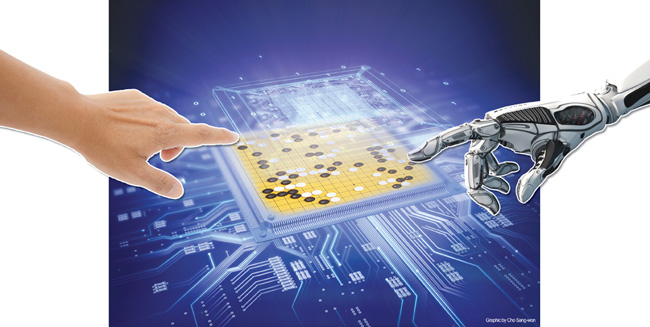
\includegraphics[width=0.8\textwidth]{figs/badukIA.jpg}
  \end{center}

  \begin{itemize}
      \item 2016: AlphaGo bat le meilleur joueur humain 
      \item Combine des méthodes de \textbf{deep learning} avec une \red{exploration d'arbre par bandit}
  \end{itemize}

}




\section{IA et Jeu de Go}




\frame{
  \frametitle{Pourquoi une IA pour le jeu de go?}

  \begin{center}
  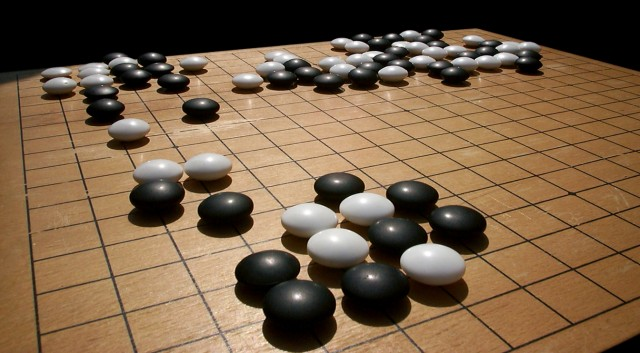
\includegraphics[width=0.5\textwidth]{figs/go-intro.jpg}
  \end{center}

  \begin{itemize}
      \item un jeu de plateau qui a longtemps résisté aux IA
      \item règles \textbf{simples}
      \item méthodes classiques (alphabeta) inefficaces
  \end{itemize}

}



\frame{
  \frametitle{Histoire}

  \begin{columns}
      \begin{column}{0.3\textwidth}
          \begin{center}
              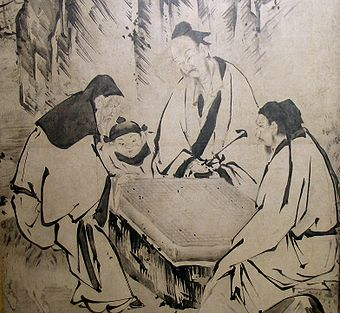
\includegraphics[width=1\textwidth]{figs/gohistory.jpg}
          \end{center}
      \end{column}
      \begin{column}{0.7\textwidth} 
          \begin{itemize}
              \item aurait été inventé en chine en 2000 BC
              \item premiers écrits: 500 BC
              \item fait parti des 4 arts majeurs chinois: peinture, calligraphie, guqin, \textit{go}
              \item se répand en Asie dès 800 dans la noblesse
              \item aujourd'hui, environ 20 millions de joueurs
          \end{itemize}
      \end{column}
  \end{columns}


}

\frame{
  \frametitle{Matériel}

  \begin{columns}
      \begin{column}{0.6\textwidth}
          \begin{itemize}
              \item plateau de jeu: Goban
              \item deux tailles 9x9 ou 19x19
              \item pierres noires et blanches 
          \end{itemize}
      \end{column}
      \begin{column}{0.4\textwidth} 
          \begin{center}
              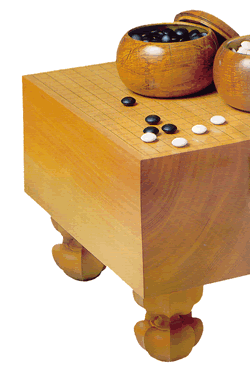
\includegraphics[width=1\textwidth]{figs/gomatos.png}
          \end{center}
      \end{column}
  \end{columns}



}

\frame{
  \frametitle{Règles: placement}

  \begin{itemize}
    \item Début de la partie: le plateau est vide
    \item Chaque joueur pose une pierre à tour de rôle
    \item Noir commence
    \item Pierres posées sur les intersections
  \end{itemize}

  \begin{center}
      \only<1> { 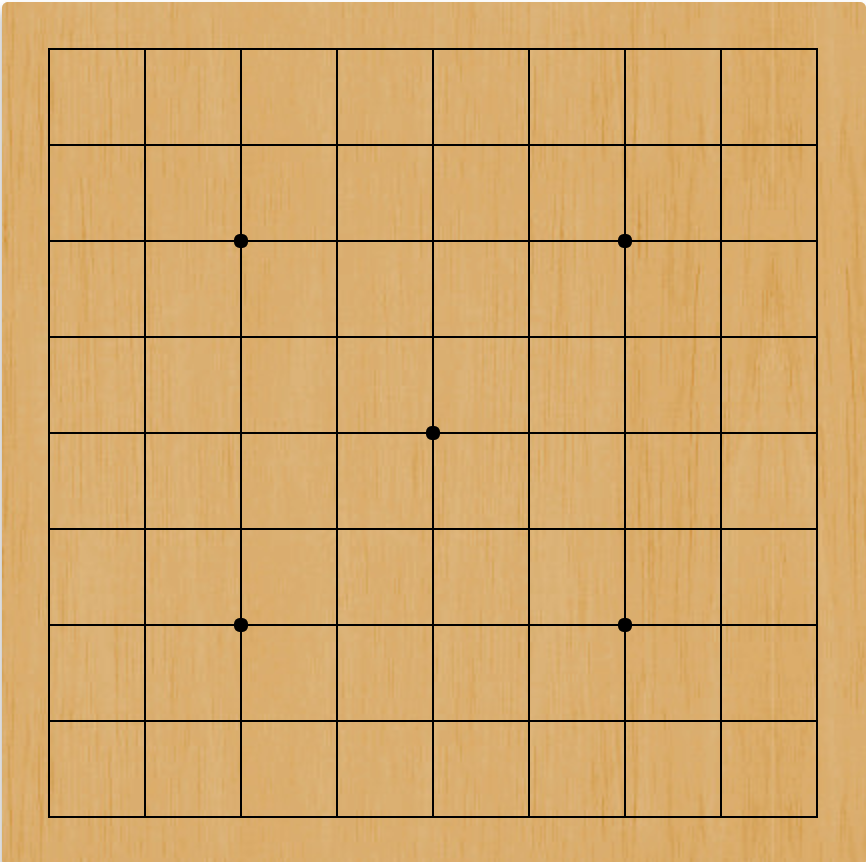
\includegraphics[width=0.4\textwidth]{figs/gorule1.png} }%
      \only<2> { 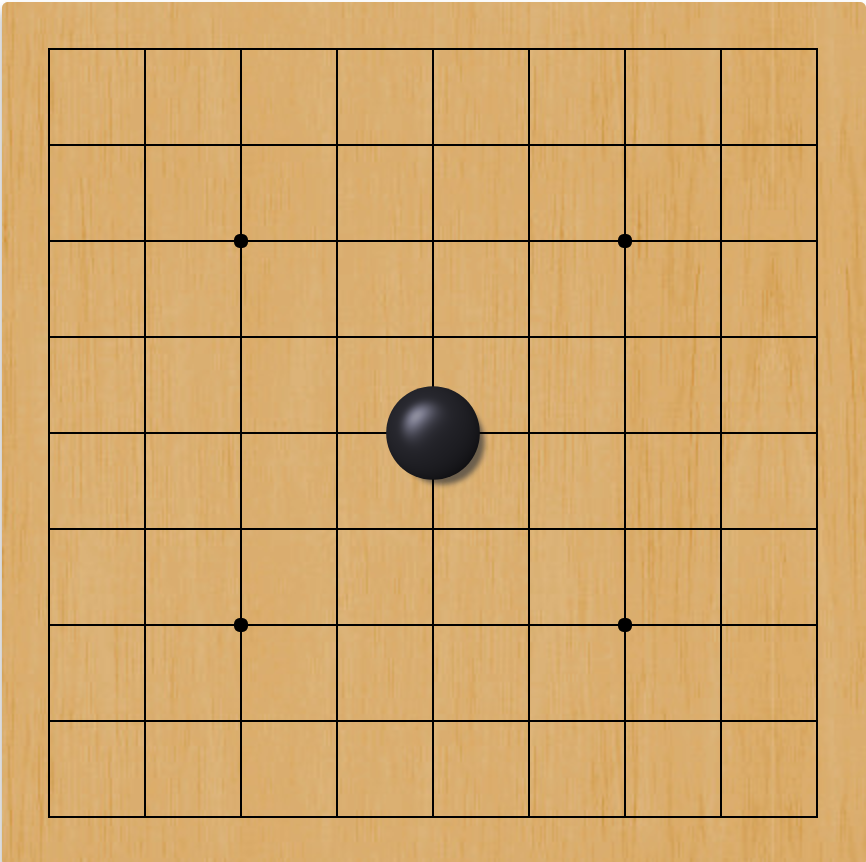
\includegraphics[width=0.4\textwidth]{figs/gorule2.png} }%
      \only<3> { 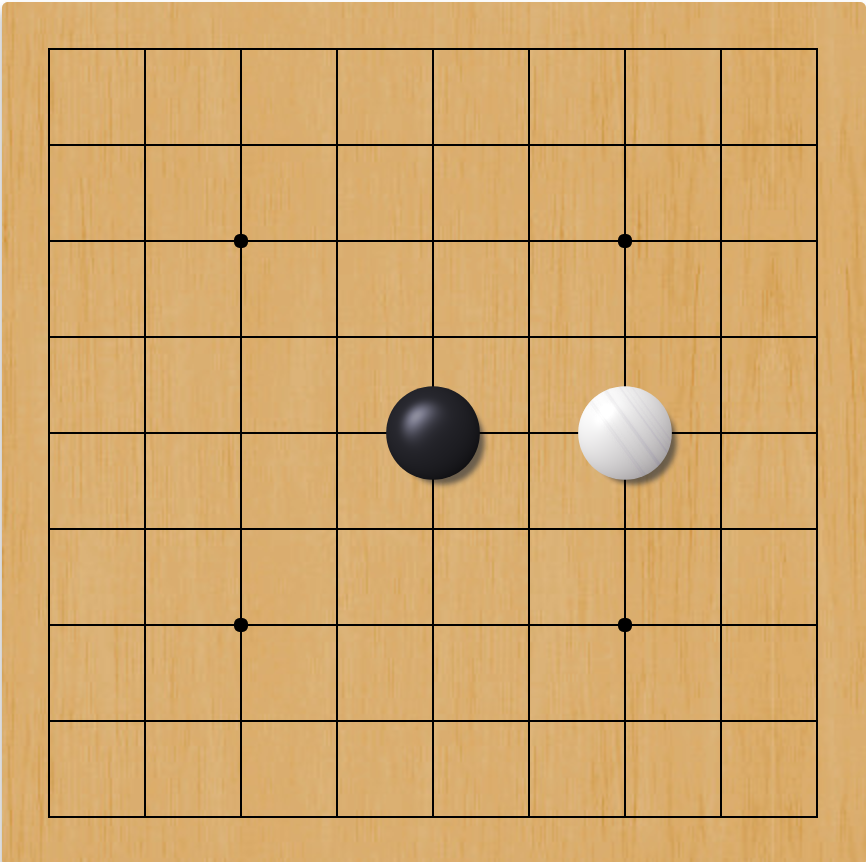
\includegraphics[width=0.4\textwidth]{figs/gorule3.png} }%
      \only<4> { 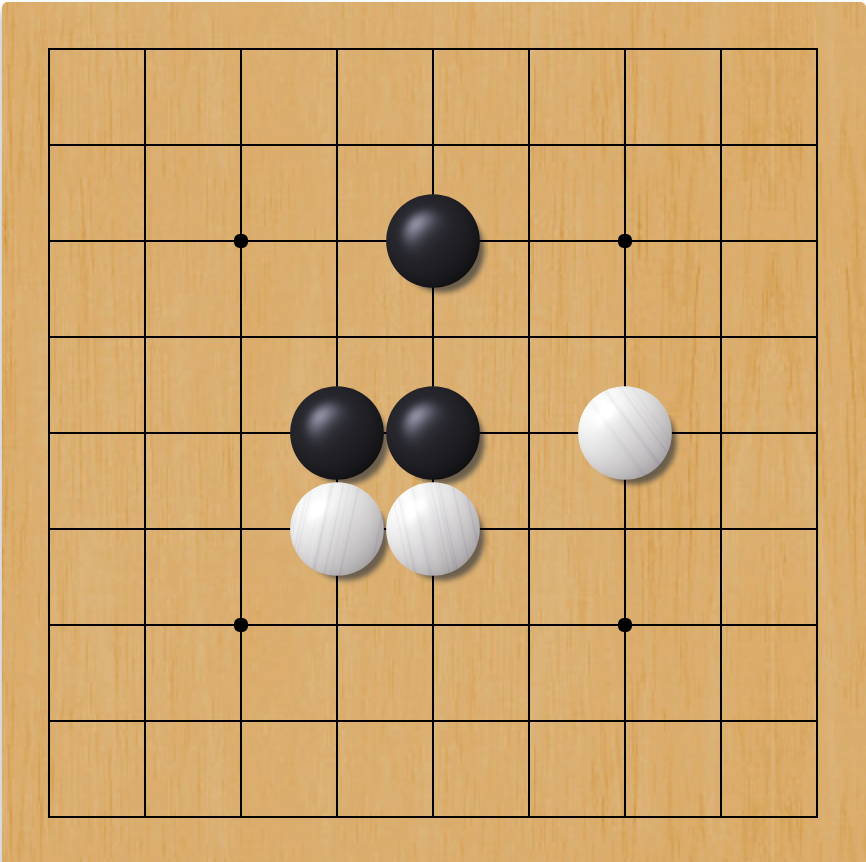
\includegraphics[width=0.4\textwidth]{figs/gorule4.png} }
  \end{center}


}

\frame{
  \frametitle{Règles: chaînes et libertés}

  \begin{itemize}
      \item Pierres reliées horizontalement ou verticalement: \textbf{une chaine}
      \item Emplacements libres autour d'une chaine: \textbf{liberté}
  \end{itemize}

  \begin{center}
      \only<1> { 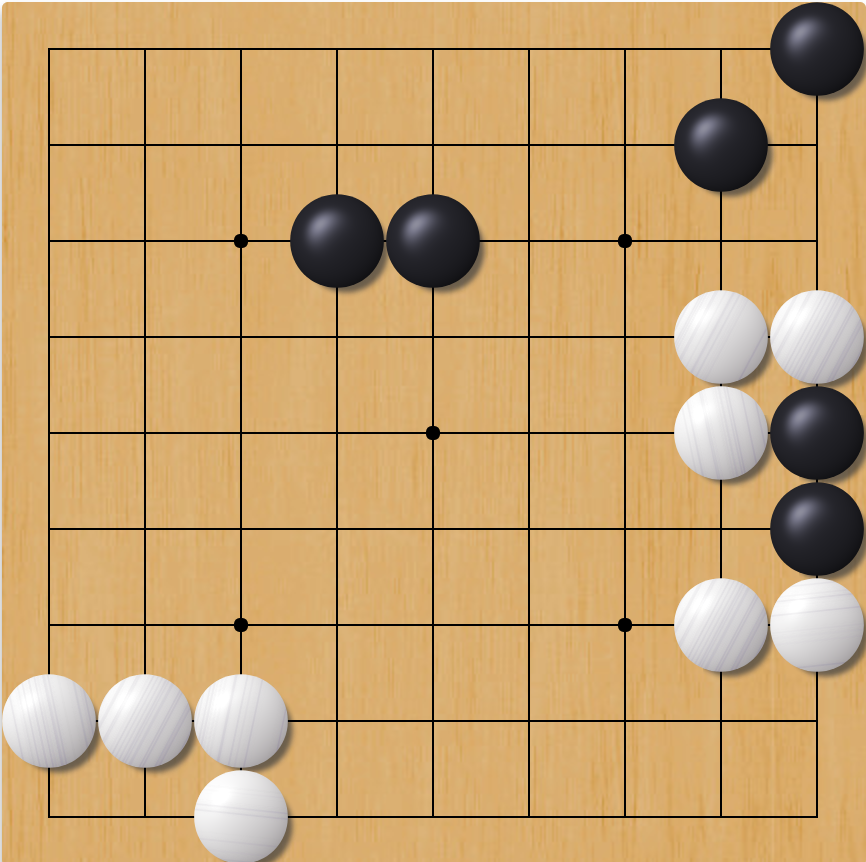
\includegraphics[width=0.4\textwidth]{figs/gorule_string1.png} }%
      \only<2> { 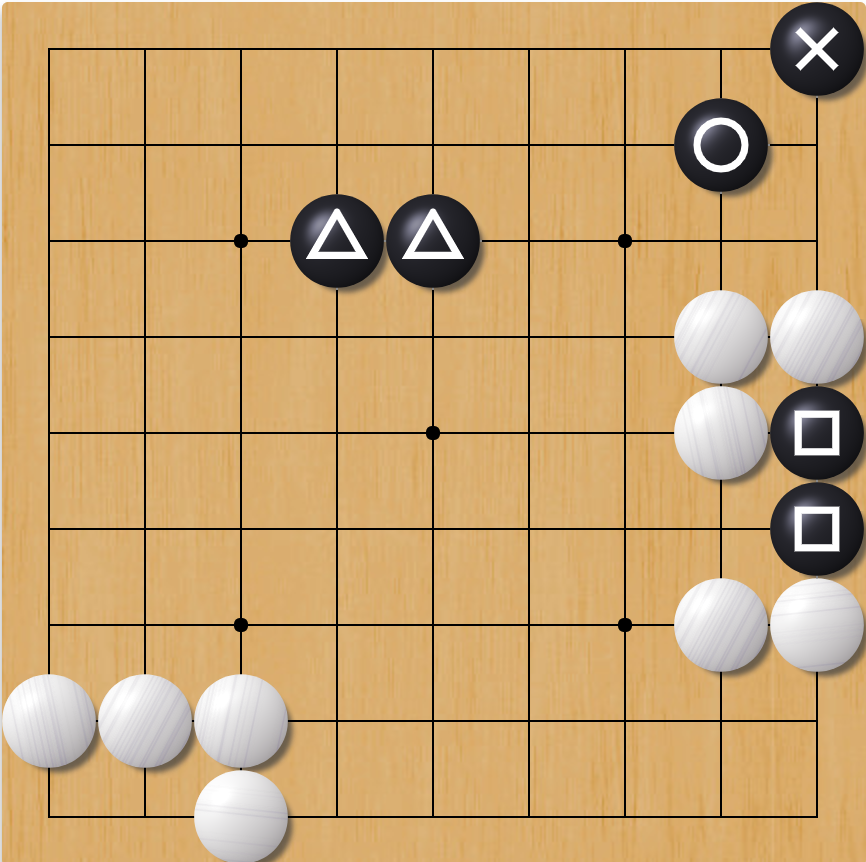
\includegraphics[width=0.4\textwidth]{figs/gorule_string2.png} }%
      \only<3> { 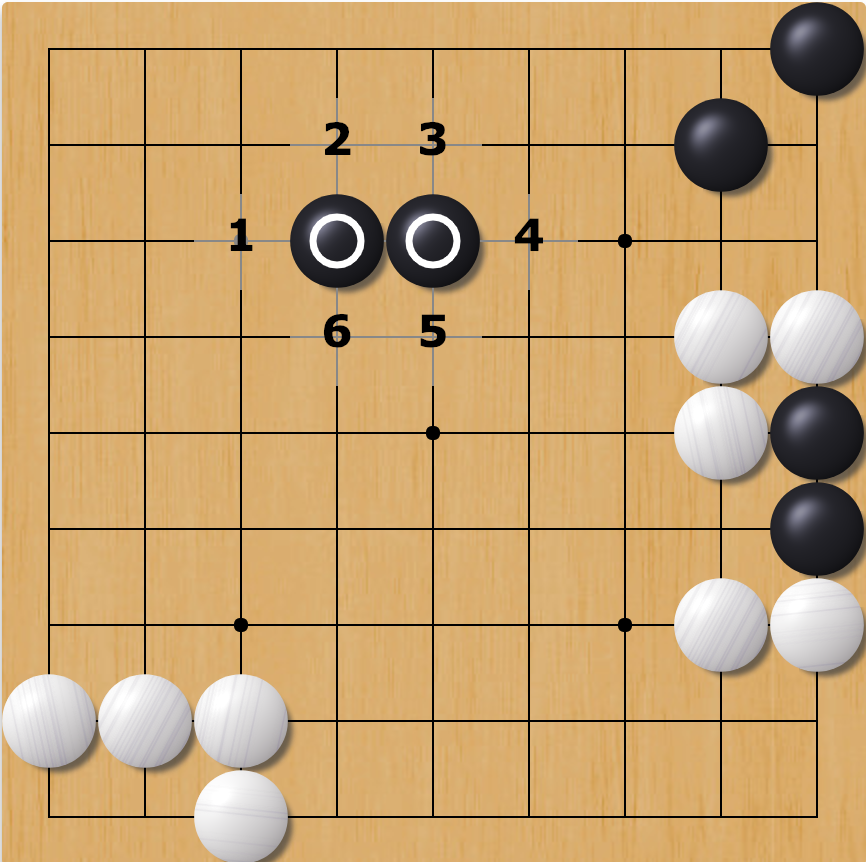
\includegraphics[width=0.4\textwidth]{figs/gorule_string3.png} }%
      \only<4> { 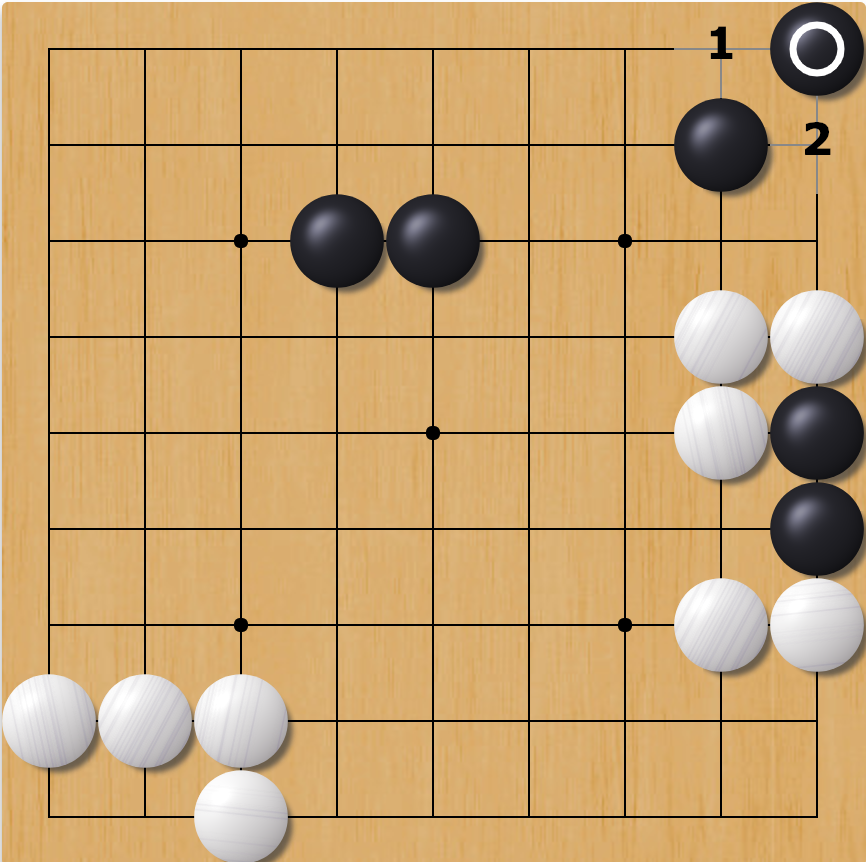
\includegraphics[width=0.4\textwidth]{figs/gorule_string4.png} }%
      \only<5> { 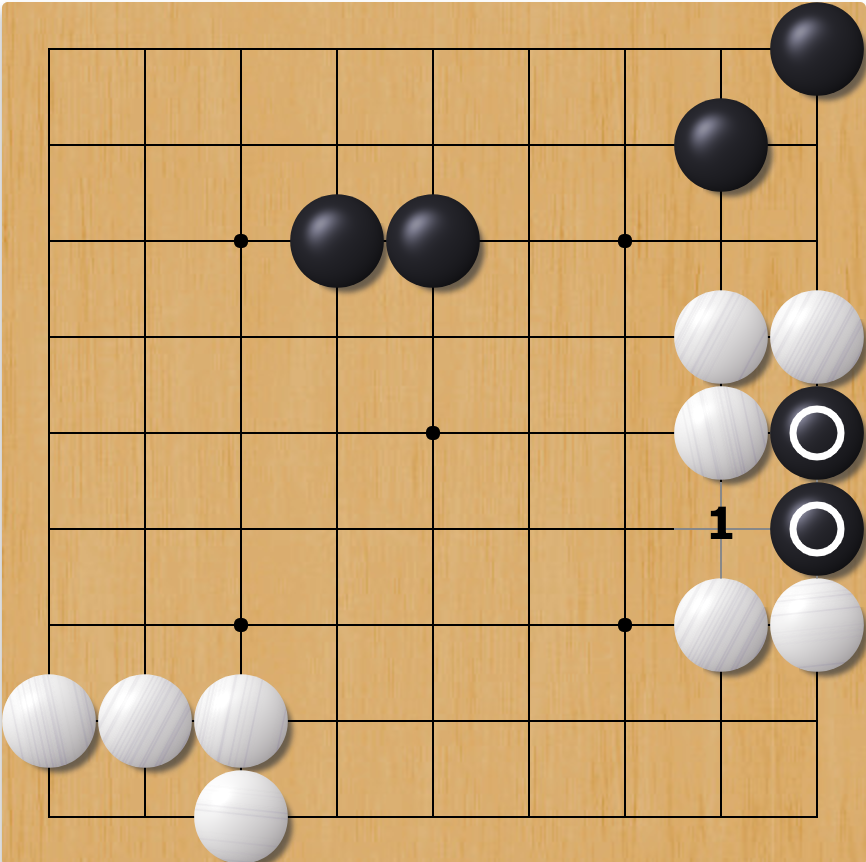
\includegraphics[width=0.4\textwidth]{figs/gorule_string5.png} }%
      \only<6> { 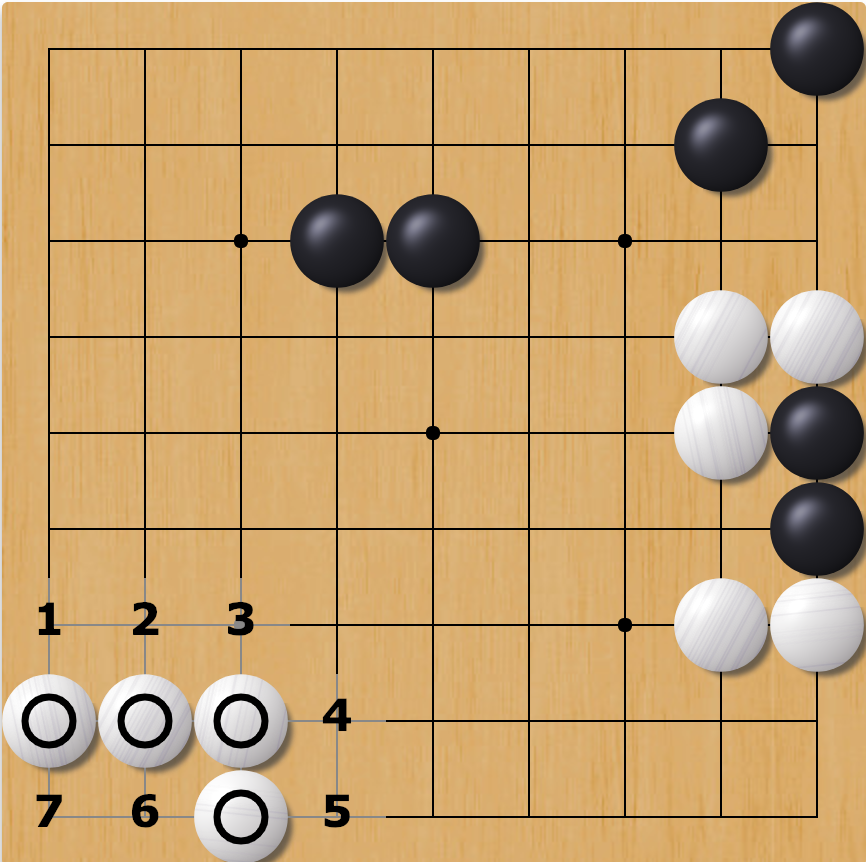
\includegraphics[width=0.4\textwidth]{figs/gorule_string6.png} }
  \end{center}

}

\frame{
  \frametitle{Règles: capture}

  \begin{itemize}
      \item Enlever la dernière liberté d'une chaine: \textbf{capture}
      \itemSo les pierres sont enlevées du plateau
  \end{itemize}

  \begin{center}
      \only<1> { 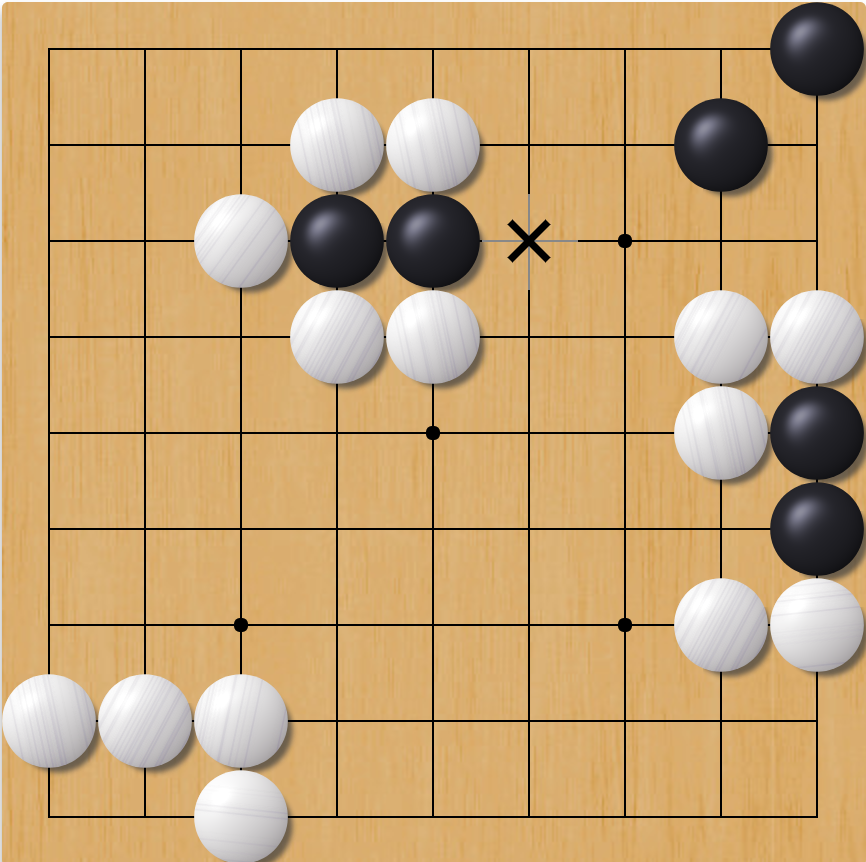
\includegraphics[width=0.4\textwidth]{figs/gorule_capture1.png} }%
      \only<2> { 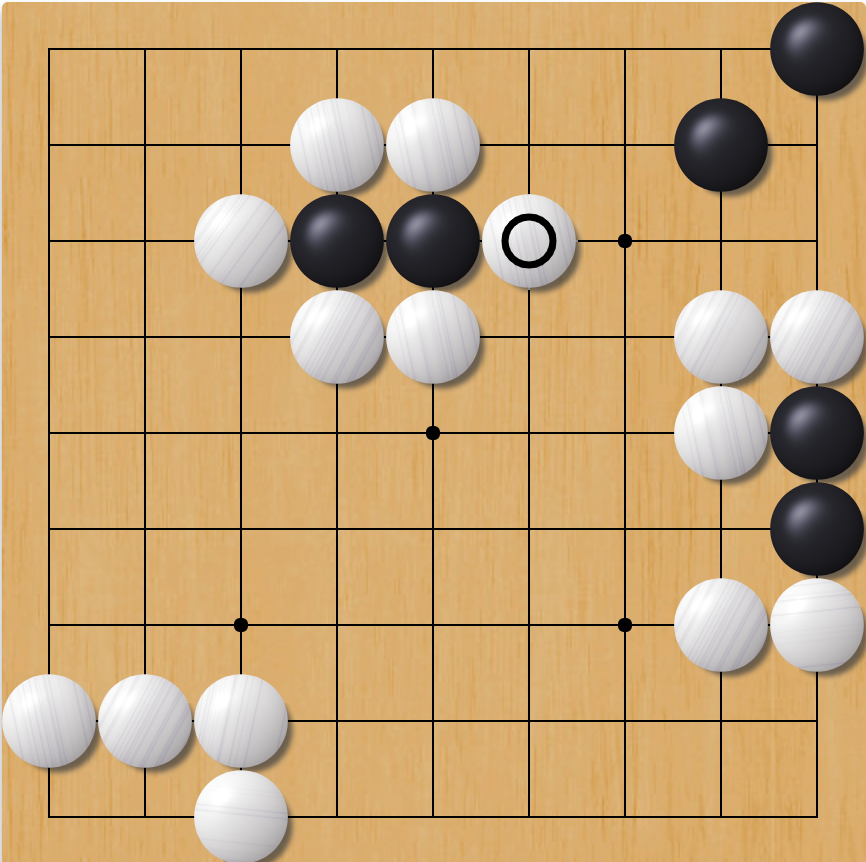
\includegraphics[width=0.4\textwidth]{figs/gorule_capture2.png} }%
      \only<3> { 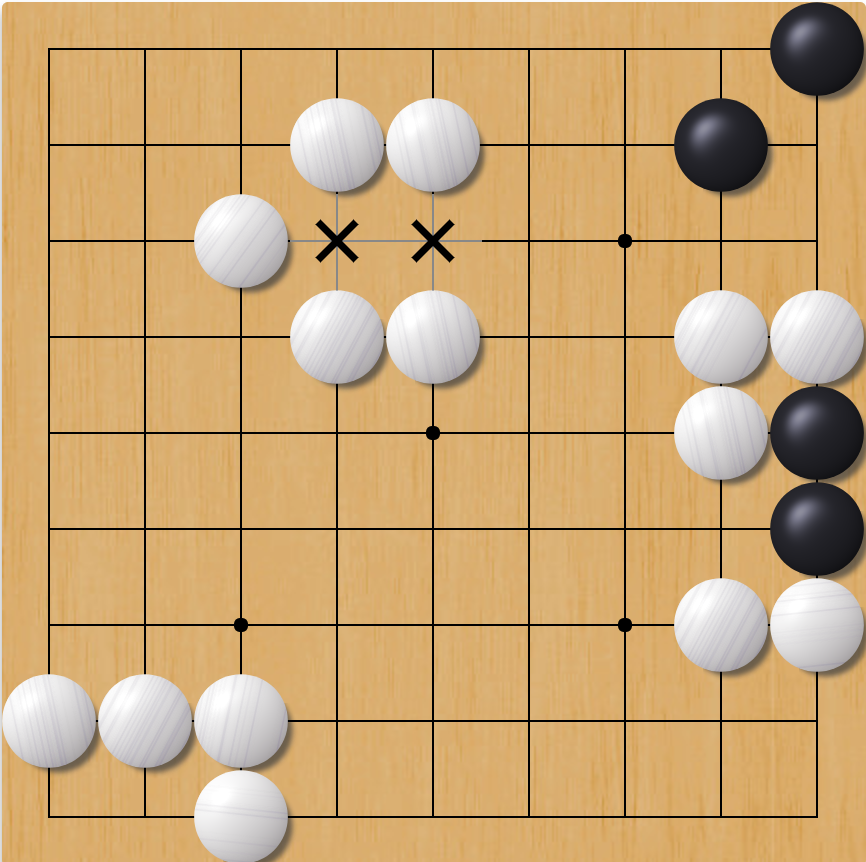
\includegraphics[width=0.4\textwidth]{figs/gorule_capture3.png} }%
      \only<4> { 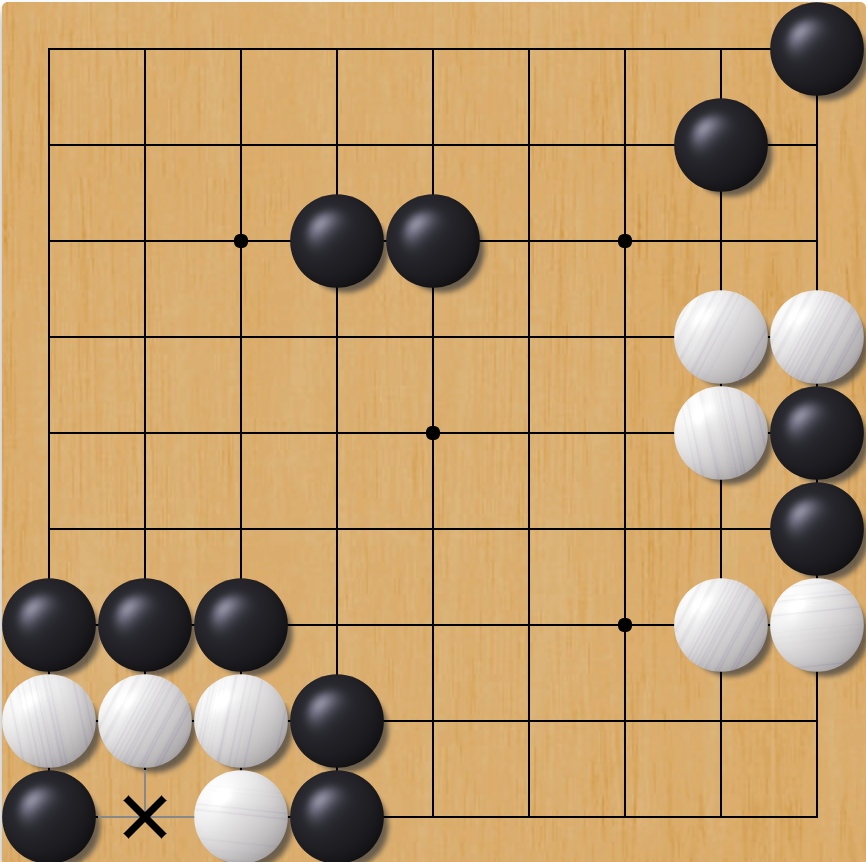
\includegraphics[width=0.4\textwidth]{figs/gorule_capture4.png} }%
      \only<5> { 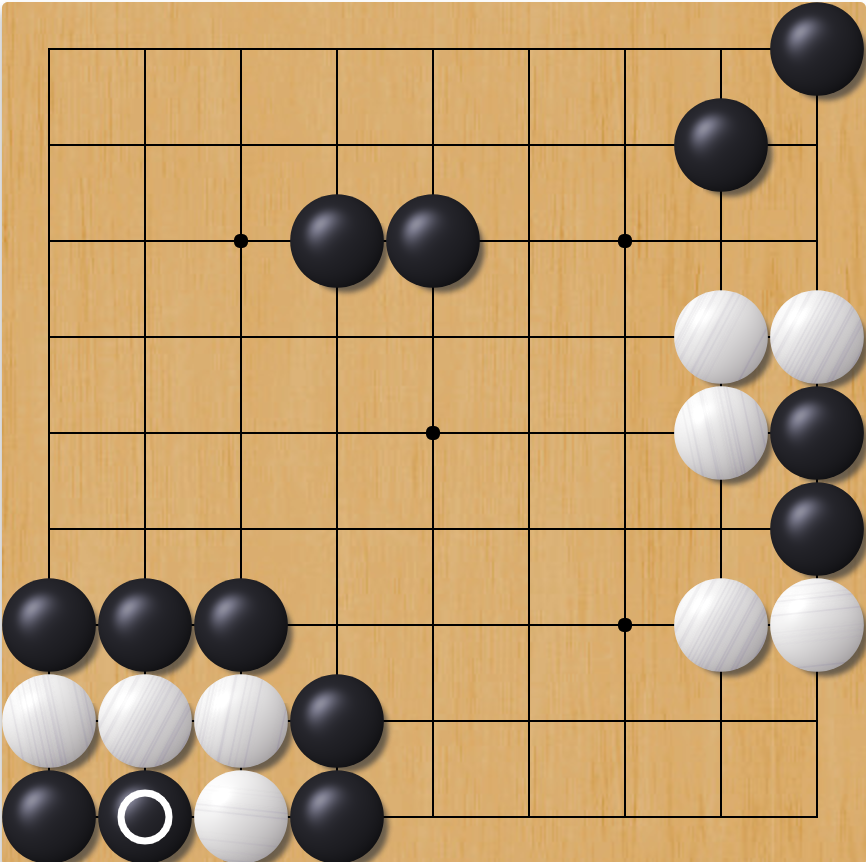
\includegraphics[width=0.4\textwidth]{figs/gorule_capture5.png} }%
      \only<6> { 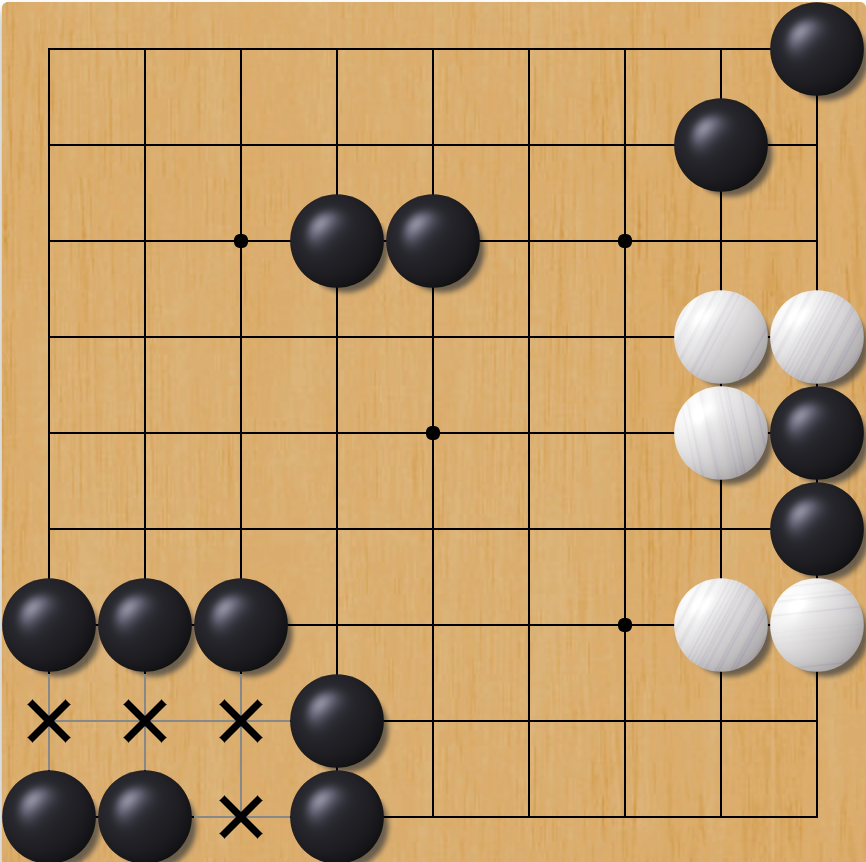
\includegraphics[width=0.4\textwidth]{figs/gorule_capture6.png} }
  \end{center}

}

\frame{
  \frametitle{Règles: fin de partie}

  \begin{itemize}
      \item partie terminée quand les deux joueurs passent
      \item score: nombre de pierres + territoire + bonus pour blanc (komi)
  \end{itemize}

  \begin{center}
      \only<1> { 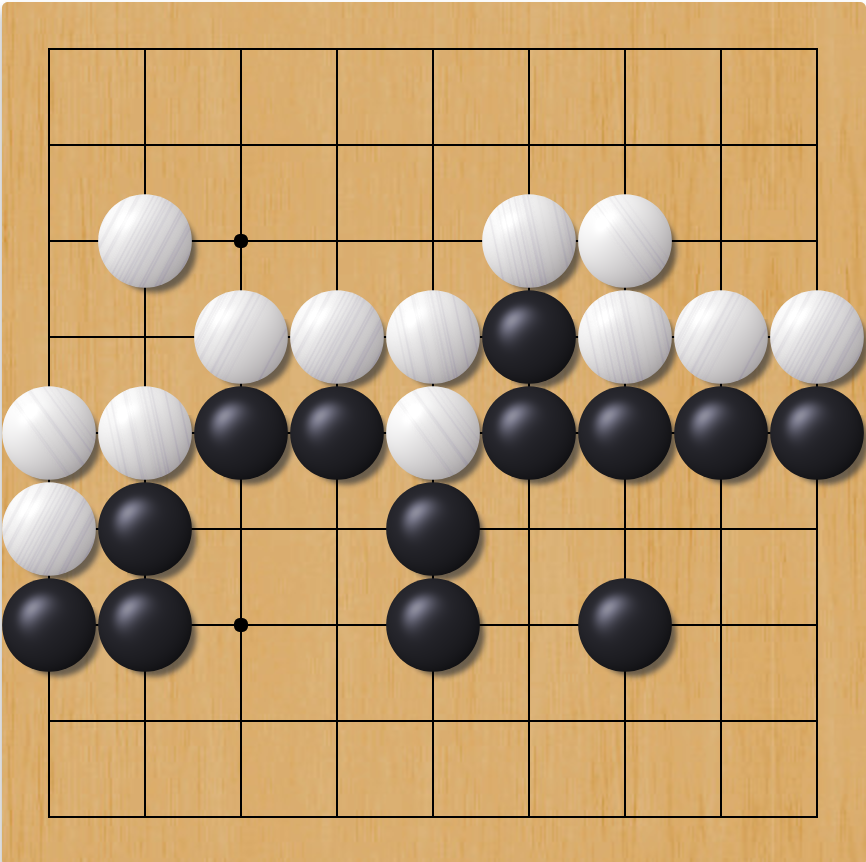
\includegraphics[width=0.4\textwidth]{figs/gorule_score1.png} }%
      \only<2> { 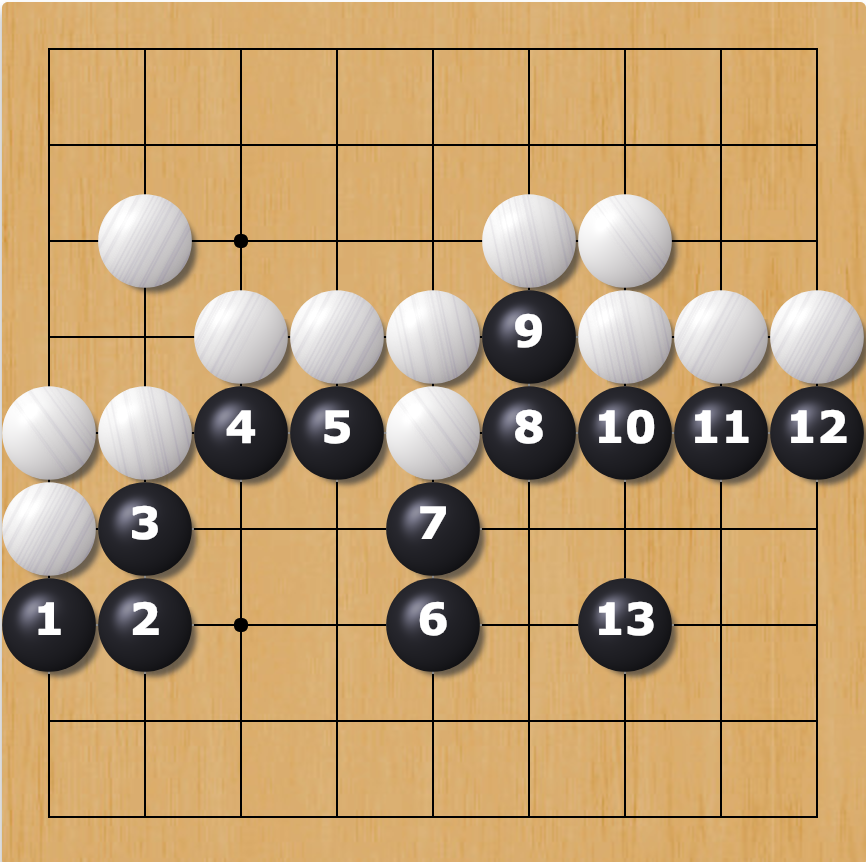
\includegraphics[width=0.4\textwidth]{figs/gorule_score2.png} }%
      \only<3> { 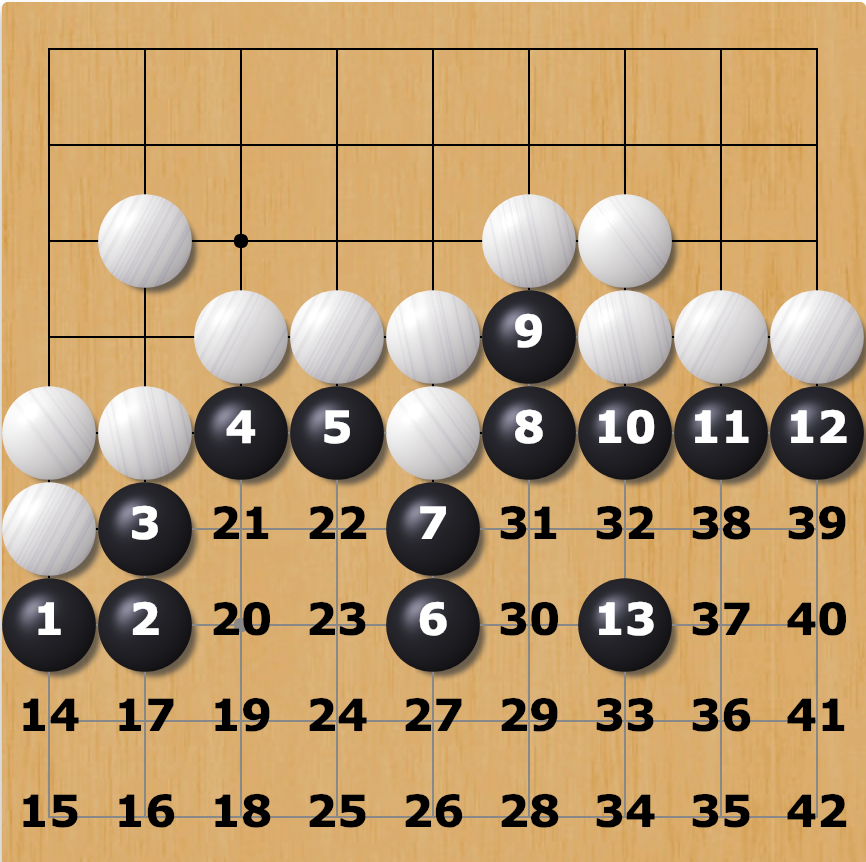
\includegraphics[width=0.4\textwidth]{figs/gorule_score3.png} }%
      \only<4> { 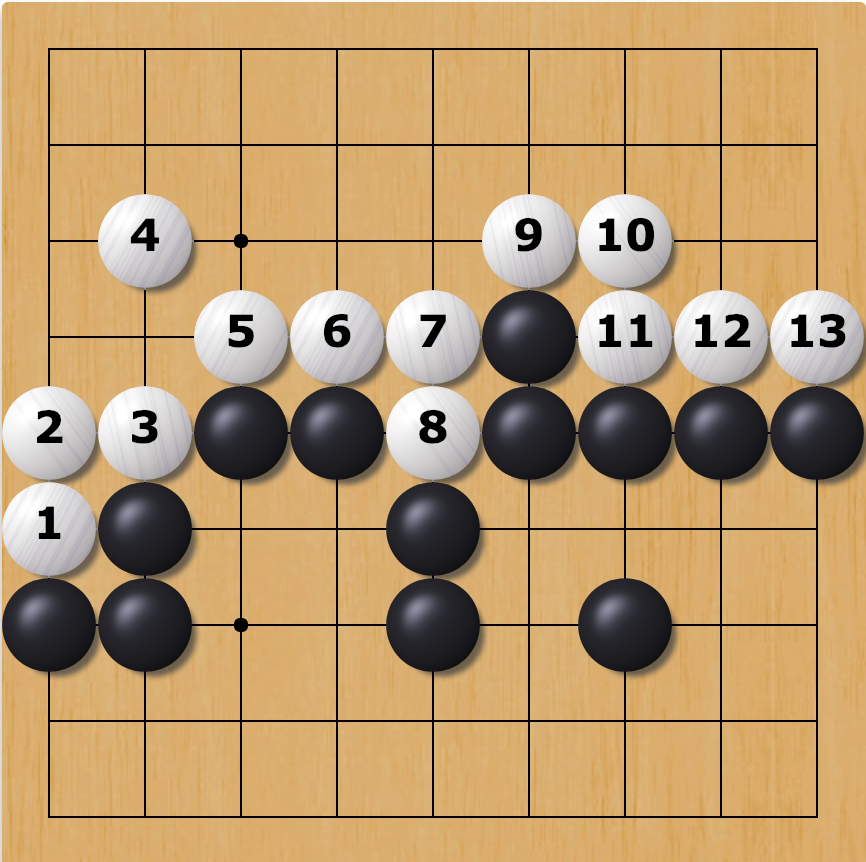
\includegraphics[width=0.4\textwidth]{figs/gorule_score4.png} }%
      \only<5> { 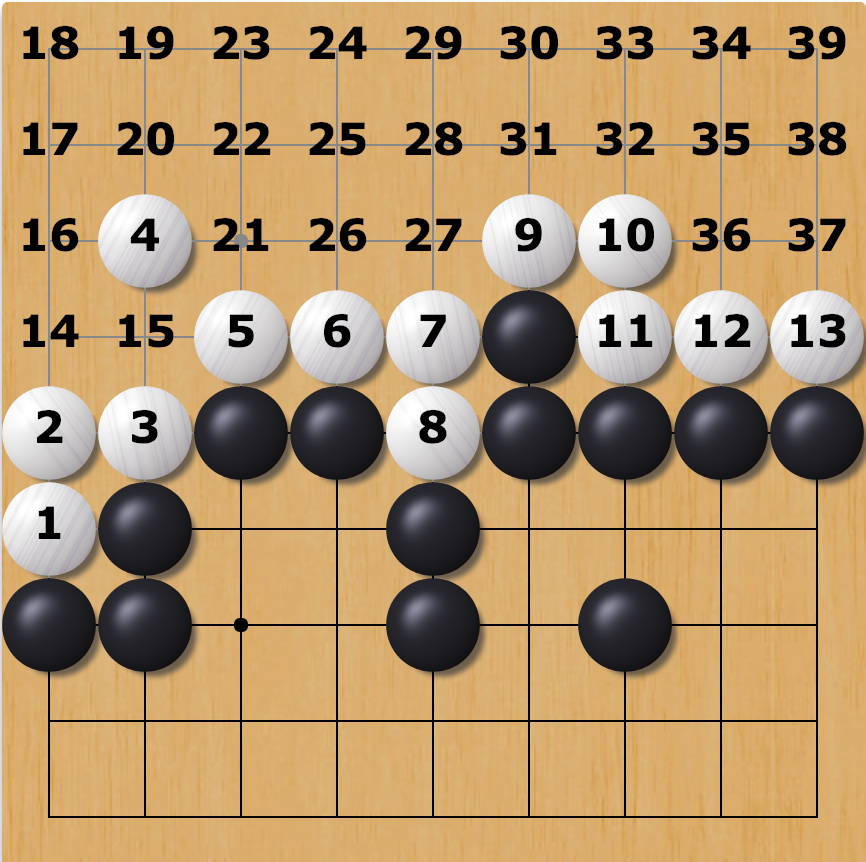
\includegraphics[width=0.4\textwidth]{figs/gorule_score5.png} }
  \end{center}
  \only<3> {score noir: 13 (pierres) + 29 (territoire)=\textbf{42}}
  \only<5> {score blanc: 13 (pierres) + 26 (territoire) + 7.5 (komi)=\textbf{46.5}}

}

\frame{
  \frametitle{Règles: le ko}


  \begin{center}
      \only<1> { 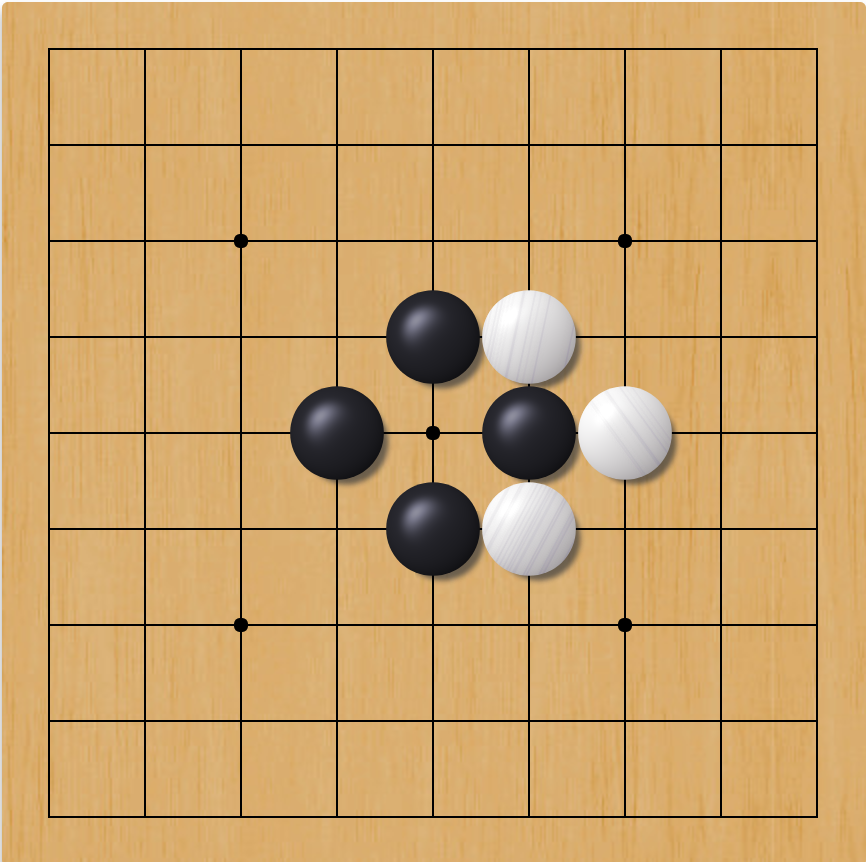
\includegraphics[width=0.4\textwidth]{figs/gorule_ko1.png} }%
      \only<2> { 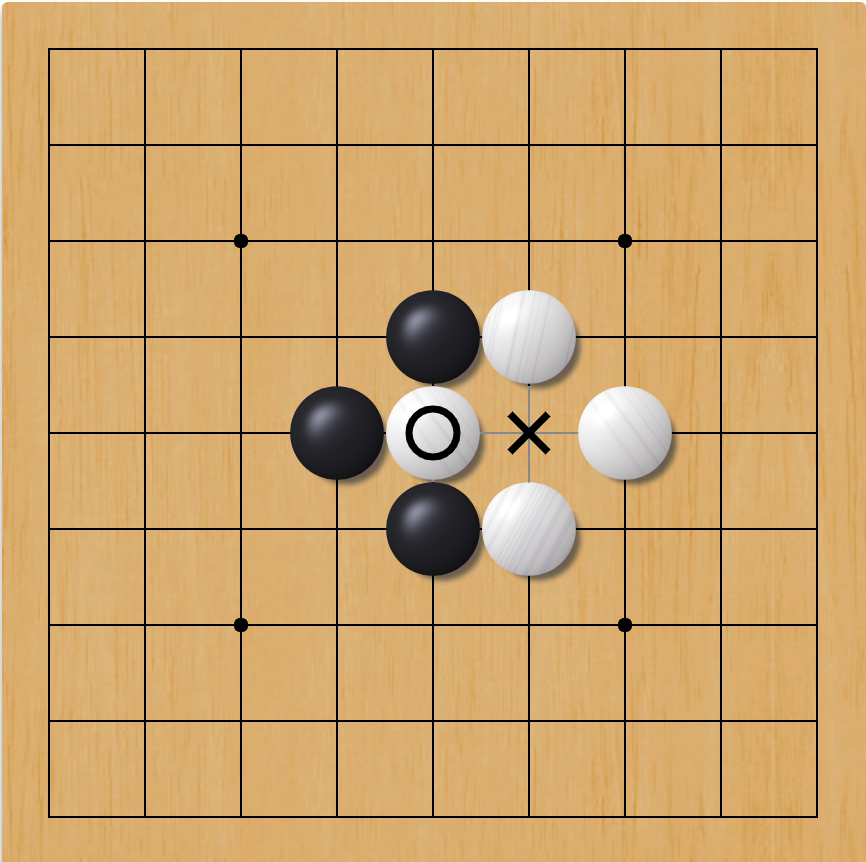
\includegraphics[width=0.4\textwidth]{figs/gorule_ko2.png} }%
      \only<3-> { 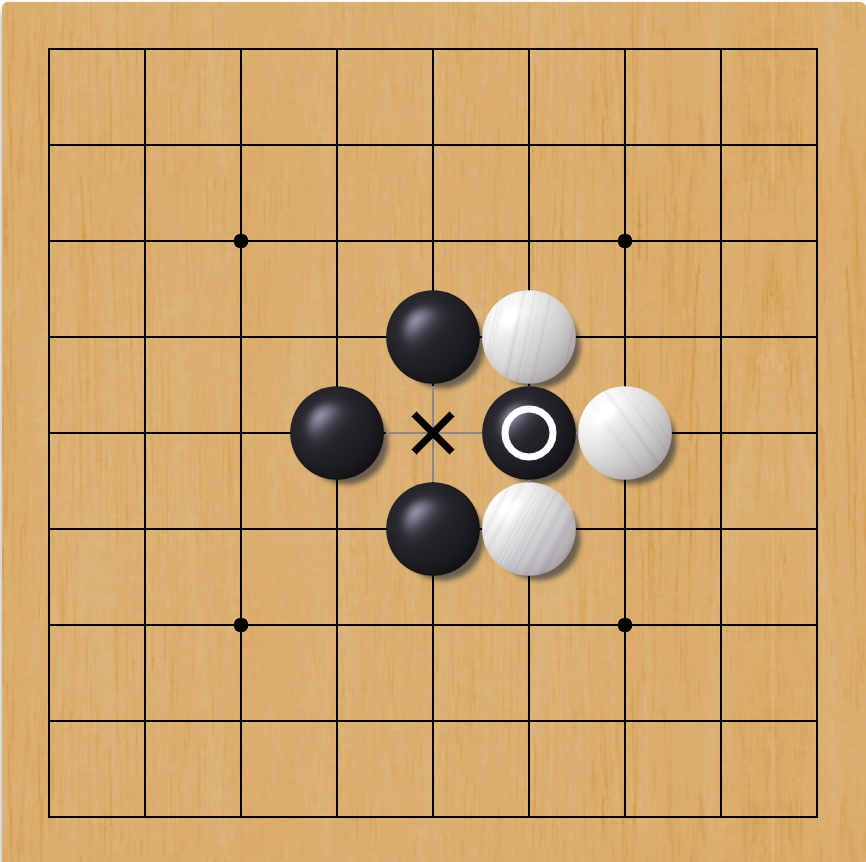
\includegraphics[width=0.4\textwidth]{figs/gorule_ko3.png} }
  \end{center}
  \only<4> {
  \begin{itemize}
      \item problème: captures répétées successives
      \item règle (humain): pas le droit de remettre le plateau dans l'état juste avant
      \item règle (ordinateur): pas le droit de remettre le plateau dans n'importe quel état précédant
  \end{itemize}

  }


}

\frame{
  \frametitle{Échelle de niveau}


\centering

\begin{tikzpicture}

    %vertical lines
    \draw [->, very thick] (0,-0.5) -- (0,5.5);
    \draw [->, very thick] (2,4) -- (2,5.5);

    %horizontal lines
    \foreach \x in {0,1,2,3,4}
        \draw [thick] (-3pt, \x) -- (3pt, \x);

    \draw [dashed] (0,4) -- (2,4);

    %nodes
    \draw (0,0) node[left=3pt] {$30$ kyu};
    \draw (0,1) node[left=3pt] {$20$ kyu};
    \draw (0,2) node[left=3pt] {$10$ kyu};
    \draw (0,2.75) node[left=3pt] {$1$ kyu};
    \draw (0,3.25) node[left=3pt] {$1$ dan};
    \draw (0,4) node[left=3pt] {$6$ dan};
    \draw (2,4) node[right=3pt] {$1$ dan};
    \draw (0,5.5) node[left=3pt] {$9$ dan};
    \draw (2,5.5) node[right=3pt] {$9$ dan};

    \draw (0,6.5) node[] {\textbf{amateur}};
    \draw (2,6.5) node[] {\textbf{pro}};

    \draw (-3,0.5) node[] {débutant};
    \draw (-3,2) node[] {moyen};
    \draw (-3,3) node[] {fort};
    \draw (-3,4) node[] {très fort};
    \draw (-3,5.5) node[] {meilleur};

\end{tikzpicture}
}


\section{Avant l'Exploration d'Arbre par Bandit}

\frame{
  \frametitle{Principe}

  \begin{itemize}
      \item Exploration d'arbre \red{alphabeta}
      \item Évaluation des nœuds basée sur des \red{connaissances expertes}
  \end{itemize}

  \begin{center}
    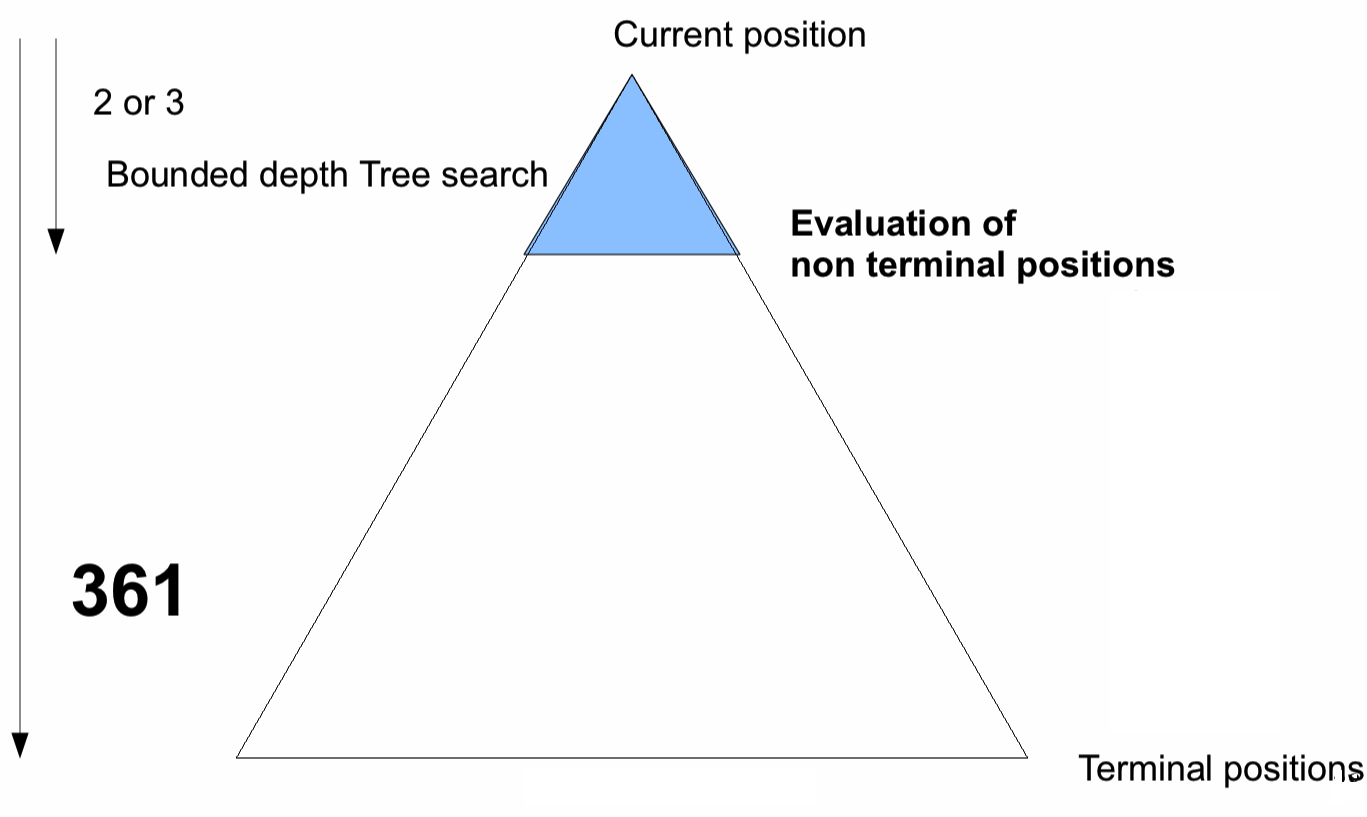
\includegraphics[width=0.8\textwidth]{figs/alphabetago.png}
  \end{center}

}

\frame{
  \frametitle{Évaluation}

  \begin{itemize}
      \item \red{Découpage} du plateau en sous parties
      \item \red{Évaluation} de chaque sous partie par \textbf{recherche locale} (souvent alphabeta)
      \itemSo groupe mort, vivant, territoire, ...
      \item \red{Recomposition} d'un score global
  \end{itemize}


}

\frame{
  \frametitle{Position à évaluer}

  \begin{center}
    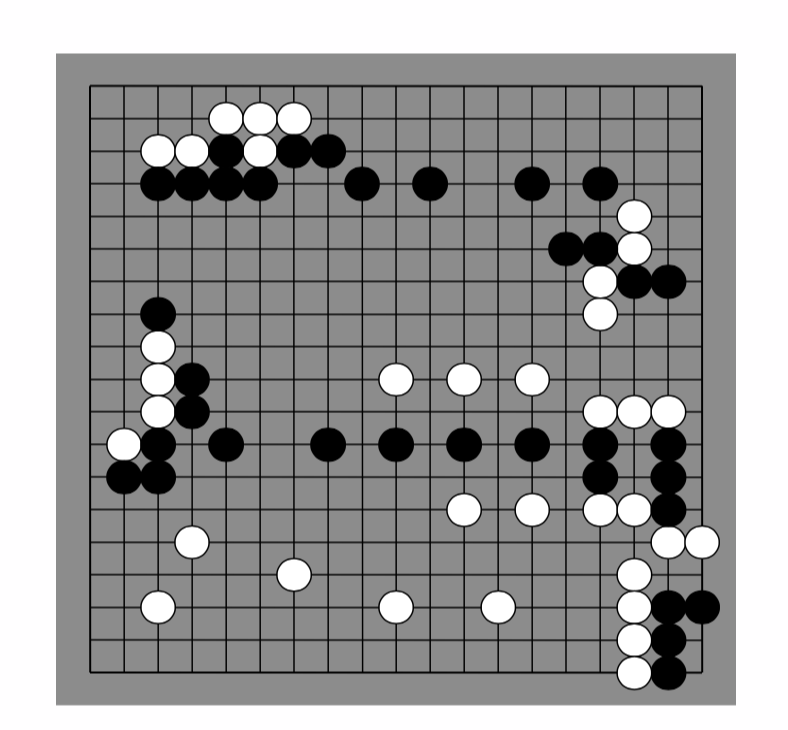
\includegraphics[width=0.7\textwidth]{figs/alphabeta_poseval.png}
  \end{center}

}

\frame{
  \frametitle{Découpage du plateau}

  \begin{center}
    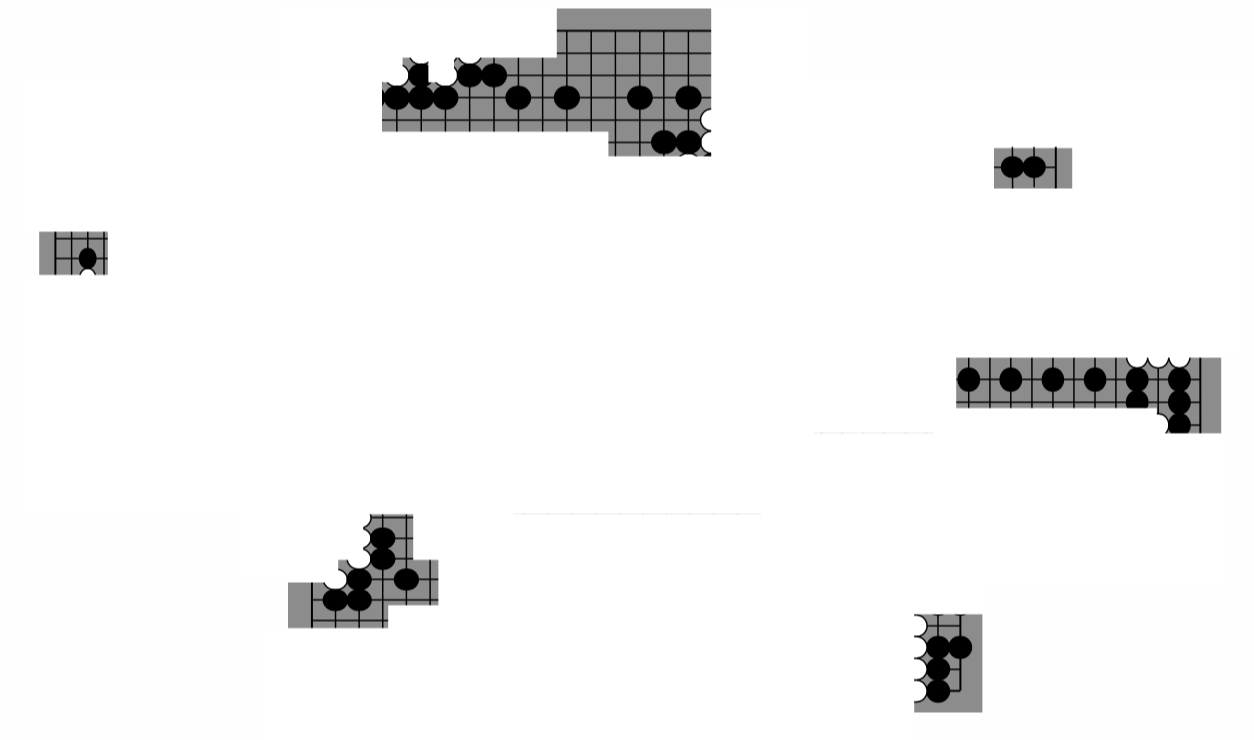
\includegraphics[width=0.8\textwidth]{figs/alphabeta_decoupage.png}
  \end{center}

}

\frame{
  \frametitle{Évaluation locale}

  \begin{center}
    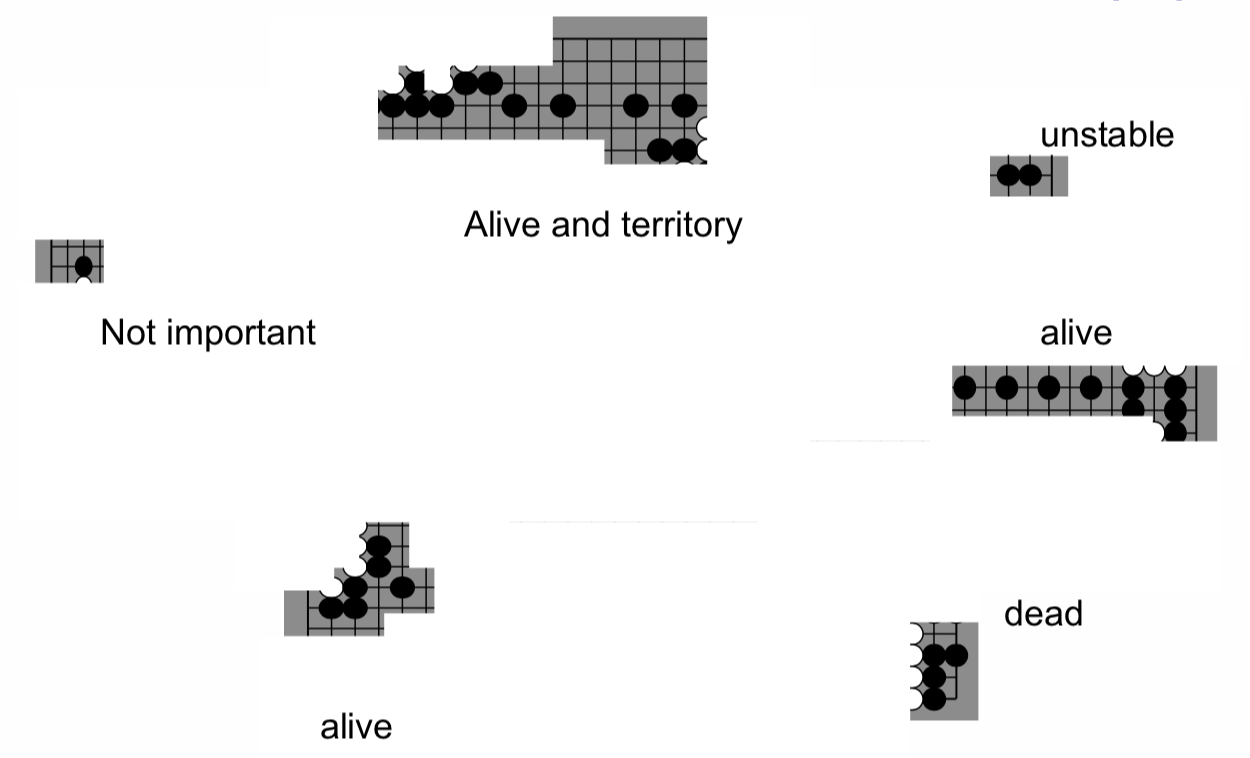
\includegraphics[width=0.8\textwidth]{figs/alphabeta_but.png}
  \end{center}

}

\frame{
  \frametitle{Évaluation globale}

  \begin{center}
    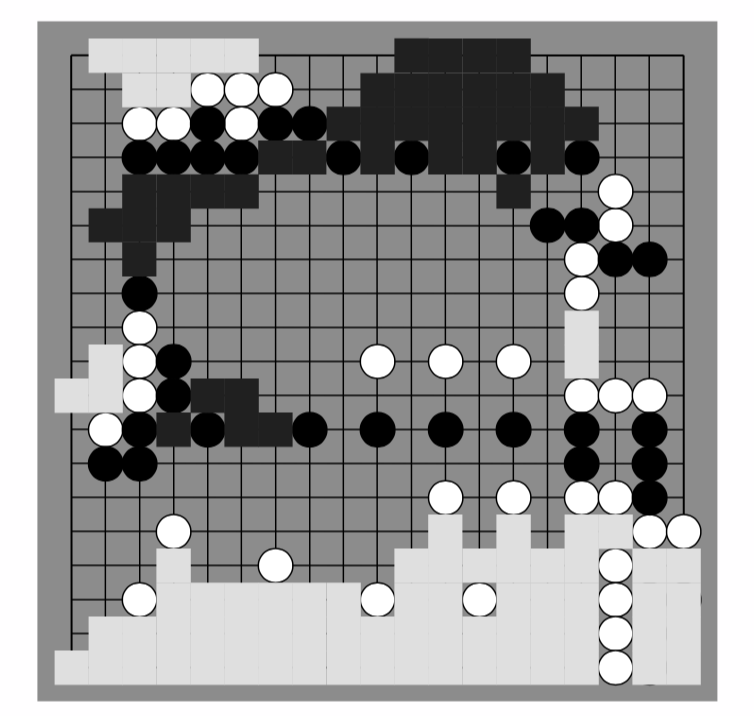
\includegraphics[width=0.7\textwidth]{figs/alphabeta_globaleval.png}
  \end{center}

}


\frame{
  \frametitle{Avantages}

  \begin{itemize}
      \item Algorithme \red{très rapide}
      \item Évaluation locale peut être très performante
  \end{itemize}

}

\frame{
  \frametitle{Inconvénients}

  \begin{itemize}
      \item Découpage et recomposition difficile et ayant un fort impact
      \item Pas d'\textbf{interaction} entre les positions locales
      \item Demande beaucoup de \textbf{connaissances expertes}
  \end{itemize}

}

\frame{
  \frametitle{Échelle de niveau}

\centering

\begin{tikzpicture}

    %vertical lines
    \draw [->, very thick] (0,-0.5) -- (0,5.5);
    \draw [->, very thick] (2,4) -- (2,5.5);

    %horizontal lines
    \foreach \x in {0,1,2,3,4}
        \draw [thick] (-3pt, \x) -- (3pt, \x);

    \draw [dashed] (0,4) -- (2,4);

    %nodes
    \draw (0,0) node[left=3pt] {$30$ kyu};
    \draw (0,1) node[left=3pt] {$20$ kyu};
    \draw (0,2) node[left=3pt] {$10$ kyu};
    \draw (0,2.75) node[left=3pt] {$1$ kyu};
    \draw (0,3.25) node[left=3pt] {$1$ dan};
    \draw (0,4) node[left=3pt] {$6$ dan};
    \draw (2,4) node[right=3pt] {$1$ dan};
    \draw (0,5.5) node[left=3pt] {$9$ dan};
    \draw (2,5.5) node[right=3pt] {$9$ dan};

    \draw (0,6.5) node[] {\textbf{amateur}};
    \draw (2,6.5) node[] {\textbf{pro}};

    \draw (-3,0.5) node[] {débutant};
    \draw (-3,2) node[] {moyen};
    \draw (-3,3) node[] {fort};
    \draw (-3,4) node[] {très fort};
    \draw (-3,5.5) node[] {meilleur};

    \draw (4,2) node[rectangle,fill=red] {} node[right=3pt,color=red] {GNU Go};

\end{tikzpicture}
}

\section{Exploration d'Arbre par Bandit}


\subsection{Construction de l'Arbre}


\frame{
  \frametitle{Idée}

  \begin{itemize}
      \item Certains coups sont très mauvais, inutile d'explorer tous leurs enfants
      \itemSo construction d'un arbre \red{déséquilibré}
      \itemSo branches plus intéressantes explorées plus profondément
      \item Construction \textbf{itérative}
  \end{itemize}

}

\frame{
  \frametitle{Principe}


  \begin{center}
    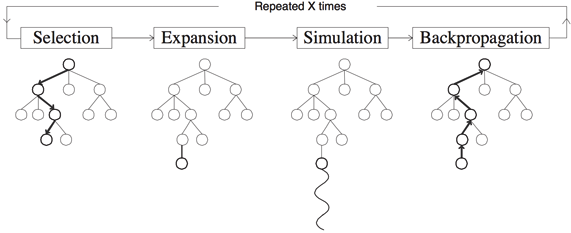
\includegraphics[width=1\textwidth]{figs/mcts-algorithm.png}
  \end{center}

}


\fi
\frame{
  \frametitle{Exemple}

\centering

\begin{tikzpicture}

    %nodes

    \onslide<1>{
        \node [very thick,circle,draw,color=blue,fill=blue!10] (as) at (0,4) {1/1};
        \node [] (ares) at (0,1) {\textbf{1}};
        \draw [thick,decorate,decoration=snake,->] (as) -- (ares);
    }
    \onslide<2->{
        \node [thick,circle,draw,color=blue] (a) at (0,4) {\only<2>{1/2}\only<3>{2/3}\only<4>{2/4}\only<5>{3/5}};
    }

    \onslide<2>{
        \node [very thick,circle,draw,color=blue,fill=blue!10] (bbs) at (2,2) {0/1};
        \draw [thick,->,color=blue] (a) -- (bbs);
        \node [] (bbres) at (2,-1) {\textbf{0}};
        \draw [thick,decorate,decoration=snake,->] (bbs) -- (bbres);
    }
    \onslide<3->{
        \node [thick,circle,draw] (bb) at (2,2) {0/1};
        \draw [thick,->] (a) -- (bb);
    }

    \onslide<3>{
        \node [very thick,circle,draw,color=blue,fill=blue!10] (bas) at (-2,2) {1/1};
        \draw [thick,->,color=blue] (a) -- (bas);
        \node [] (bares) at (-2,-1) {\textbf{1}};
        \draw [thick,decorate,decoration=snake,->] (bas) -- (bares);
    }
    \onslide<4->{
        \node [thick,circle,draw,color=blue] (ba) at (-2,2) {\only<4>{1/2}\only<5>{2/3}}; 
        \draw [thick,->,color=blue] (a) -- (ba);
    }

    \onslide<4>{
        \node [very thick,circle,draw,color=blue,fill=blue!10] (cas) at (-3,0) {0/1};
        \draw [thick,->,color=blue] (ba) -- (cas);
        \node [] (cares) at (-3,-3) {\textbf{0}};
        \draw [thick,decorate,decoration=snake,->] (cas) -- (cares);
    }
    \onslide<5->{
        \node [thick,circle,draw] (ca) at (-3,0) {0/1};
        \draw [thick,->] (ba) -- (ca);
    }

    \onslide<5>{
        \node [very thick,circle,draw,color=blue,fill=blue!10] (cbs) at (-1,0) {1/1};
        \draw [thick,->,color=blue] (ba) -- (cbs);
        \node [] (cbres) at (-1,-3) {\textbf{1}};
        \draw [thick,decorate,decoration=snake,->] (cbs) -- (cbres);
    }
    %\onslide<5->{
    %    \node [thick,circle,draw] (cb) at (-1,0) {1/1};
    %    \draw [thick,->] (ba) -- (cb);
    %}

\end{tikzpicture}
}

\frame{
  \frametitle{Exemple}

\centering

\begin{tikzpicture}

    %nodes

    \node [thick,circle,draw,color=blue] (a) at (0,4) {3/5};

        \node [thick,circle,draw] (bb) at (2,2) {0/1};
        \draw [thick,->] (a) -- (bb);

        \node [thick,circle,draw,color=blue] (ba) at (-2,2) {2/3}; 
        \draw [thick,->,color=blue] (a) -- (ba);

        \node [thick,circle,draw] (ca) at (-3,0) {0/1};
        \draw [thick,->] (ba) -- (ca);

        \node [very thick,circle,draw,color=blue,fill=blue!10] (cbs) at (-1,0) {1/1};
        \draw [thick,->,color=blue] (ba) -- (cbs);
        \node [] (cbres) at (-1,-3) {\textbf{1}};
        \draw [thick,decorate,decoration=snake,->] (cbs) -- (cbres);

        \node [color=blue] at (-3,3.5) {\textbf{Descente}};
        \node [] at (0.5,-1.5) {\textbf{Évaluation}};
\end{tikzpicture}
}

\iftrue


\frame{
  \frametitle{Évaluation}

  \textbf{Monte Carlo}
  \begin{itemize}
      \item Choix \red{aléatoire} d'un coup jusqu'à la fin de la partie
  \end{itemize}

  Propriétés
  \begin{itemize}
      \item méthode générique
      \item facile à implémenter
      \item \textbf{non biaisé}
      \item possibilité d'intégrer des connaissances expertes en utilisant une distribution non uniforme
  \end{itemize}
  A l'origine du nom \textbf{Monte Carlo Tree Search} mais cette évaluation peut être remplacée

}


\subsection{Problème de Bandit}

\begin{frame}
    \frametitle{Introduction du problème}
    \begin{center}
        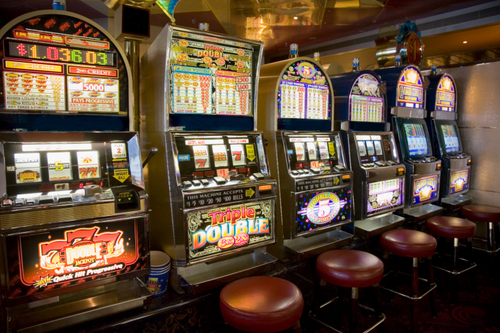
\includegraphics[scale=0.8]{figs/bandit_casino.jpg}
    \end{center}
    Dans un casino, il y a plusieurs machines à sous différentes en terme de récompense.
    \begin{itemize}
        \item Comment répartir mes pièces entre les machines?
    \end{itemize}
\end{frame}

\begin{frame}
    \frametitle{Autres problèmes similaires}
    \begin{center}
        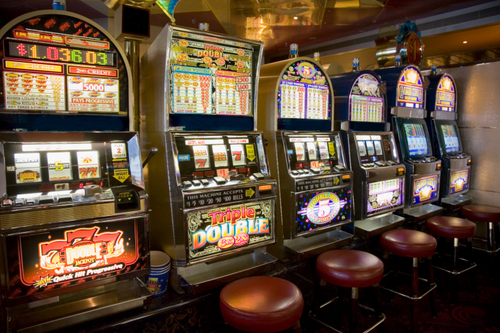
\includegraphics[scale=0.8]{figs/bandit_casino.jpg}
    \end{center}
    \begin{itemize}
        \item Essais cliniques: trouver le traitement qui fonctionne le mieux.
        \item Sélection d'un serveur dans un réseau: trouver le serveur avec le temps de réponse le plus faible.
        \item Publicité ciblée: trouver le type de pub qui intéressera le plus un utilisateur.
        \item ...
    \end{itemize}
    Ce sont des problèmes où on a plusieurs fois le même choix à effectuer. Le choix conduit à une récompense aléatoire.
\end{frame}


\begin{frame}
    \frametitle{Définition formelle}
    \begin{center}
        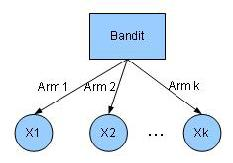
\includegraphics[scale=0.5]{figs/bandit.jpg}
    \end{center}
    \begin{itemize}
        \item un ensemble de bras $A=\{1,...,K\}$.
        \item chaque bras est associé à une distribution de probabilité $X_k$ d'espérance $\mu_k$.
        \item l'algorithme choisit un bras $a$ à chaque pas de temps.
        \item le bandit retourne une récompense $r$ : une réalisation de $X_a$.
        \item les tirages successifs sur un même bras sont indépendant et identiquement distribués.
    \end{itemize}
\end{frame}



\begin{frame}
    \frametitle{Notations supplémentaires}
    \begin{itemize}
        \item $T_i(n)$: le nombre de fois que le bras $i$ a été sélectionné au pas de temps $n$.
        \item $\mu^* = \max_{1 \le i \le K}\mu_i$
        \item $\Delta_i = \mu^* - \mu_i$ 
        \item $\Delta = \min_{i:\Delta_i > 0}\Delta_i$
    \end{itemize}


\end{frame}


\begin{frame}
    \frametitle{Objectif}

    Le but est d'optimiser le regret $R_n$ défini comme suit:

    $$R_n=\mu^*n - \mathbb{E} \sum_{j=1}^{K}  T_j(n) \mu_j$$
    $$R_n=\sum_{j=1}^{K} \Delta_j \mathbb{E} [T_j(n)]$$

\end{frame}



\begin{frame}
    \frametitle{Borne inférieure}


    Pour toute stratégie d'allocation et pour tout bras non optimal:
    $$\mathbb{E} [T_j(n)] \ge \frac{\log n}{D(p_j || p^*)}$$

    $$\mbox{où }D(p_j || p^*) = \int p_j \log \frac{p_j}{p^*}$$
    On en déduit que le meilleur regret atteignable est en ${\color{red} \log(n)}$.

    \hfill [Lai and Robbins, 1985]

\end{frame}



\begin{frame}
    \frametitle{UCB}
    Principe de l'algorithme:
    \begin{itemize}
        \item A partir des informations disponibles au temps $t$, on calcule la borne de confiance supérieur (UCB) correspondant à chaque bras.
        \item On choisit le bras qui a la valeur UCB la plus grande.
    \end{itemize}
    \hfill [Auer and all, 2002]
\end{frame}

\begin{frame}
    \frametitle{UCB}
    Calcul de la valeur UCB pour le bras $i$ au pas de temps $t$:
    $$ {\color{red} \hat{\mu}_{i,t-1}} + {\color{green} \sqrt{\frac{3\log(t)}{2T_i(t-1)}}} $$
    où $\hat{\mu}_{i,t-1} $ correspond à la moyenne empirique du bras $i$.
    
\end{frame}

\begin{frame}
    \frametitle{UCB}
    Borne sur le regret:
    $$ R_n \le 6*\sum_{i \ne i^*}\frac{\color{red}\log(n)}{\Delta_i} + K(\frac{\pi^2}{3}+1) $$
    
\end{frame}


\frame{
  \frametitle{Rappel}

\centering

\begin{tikzpicture}

    %nodes

    \node [thick,circle,draw,color=blue] (a) at (0,4) {3/5};

        \node [thick,circle,draw] (bb) at (2,2) {0/1};
        \draw [thick,->] (a) -- (bb);

        \node [thick,circle,draw,color=blue] (ba) at (-2,2) {2/3}; 
        \draw [thick,->,color=blue] (a) -- (ba);

        \node [thick,circle,draw] (ca) at (-3,0) {0/1};
        \draw [thick,->] (ba) -- (ca);

        \node [very thick,circle,draw,color=blue,fill=blue!10] (cbs) at (-1,0) {1/1};
        \draw [thick,->,color=blue] (ba) -- (cbs);
        \node [] (cbres) at (-1,-3) {\textbf{1}};
        \draw [thick,decorate,decoration=snake,->] (cbs) -- (cbres);

        \node [color=blue] at (-3,3.5) {\textbf{Descente}};
        \node [] at (0.5,-1.5) {\textbf{Évaluation}};
\end{tikzpicture}
}




\begin{frame}
    \frametitle{Descente dans l'arbre}
    La descente dans l'arbre se fait en considérant que chaque choix d'une branche est un problème de bandit.

    \begin{center}
        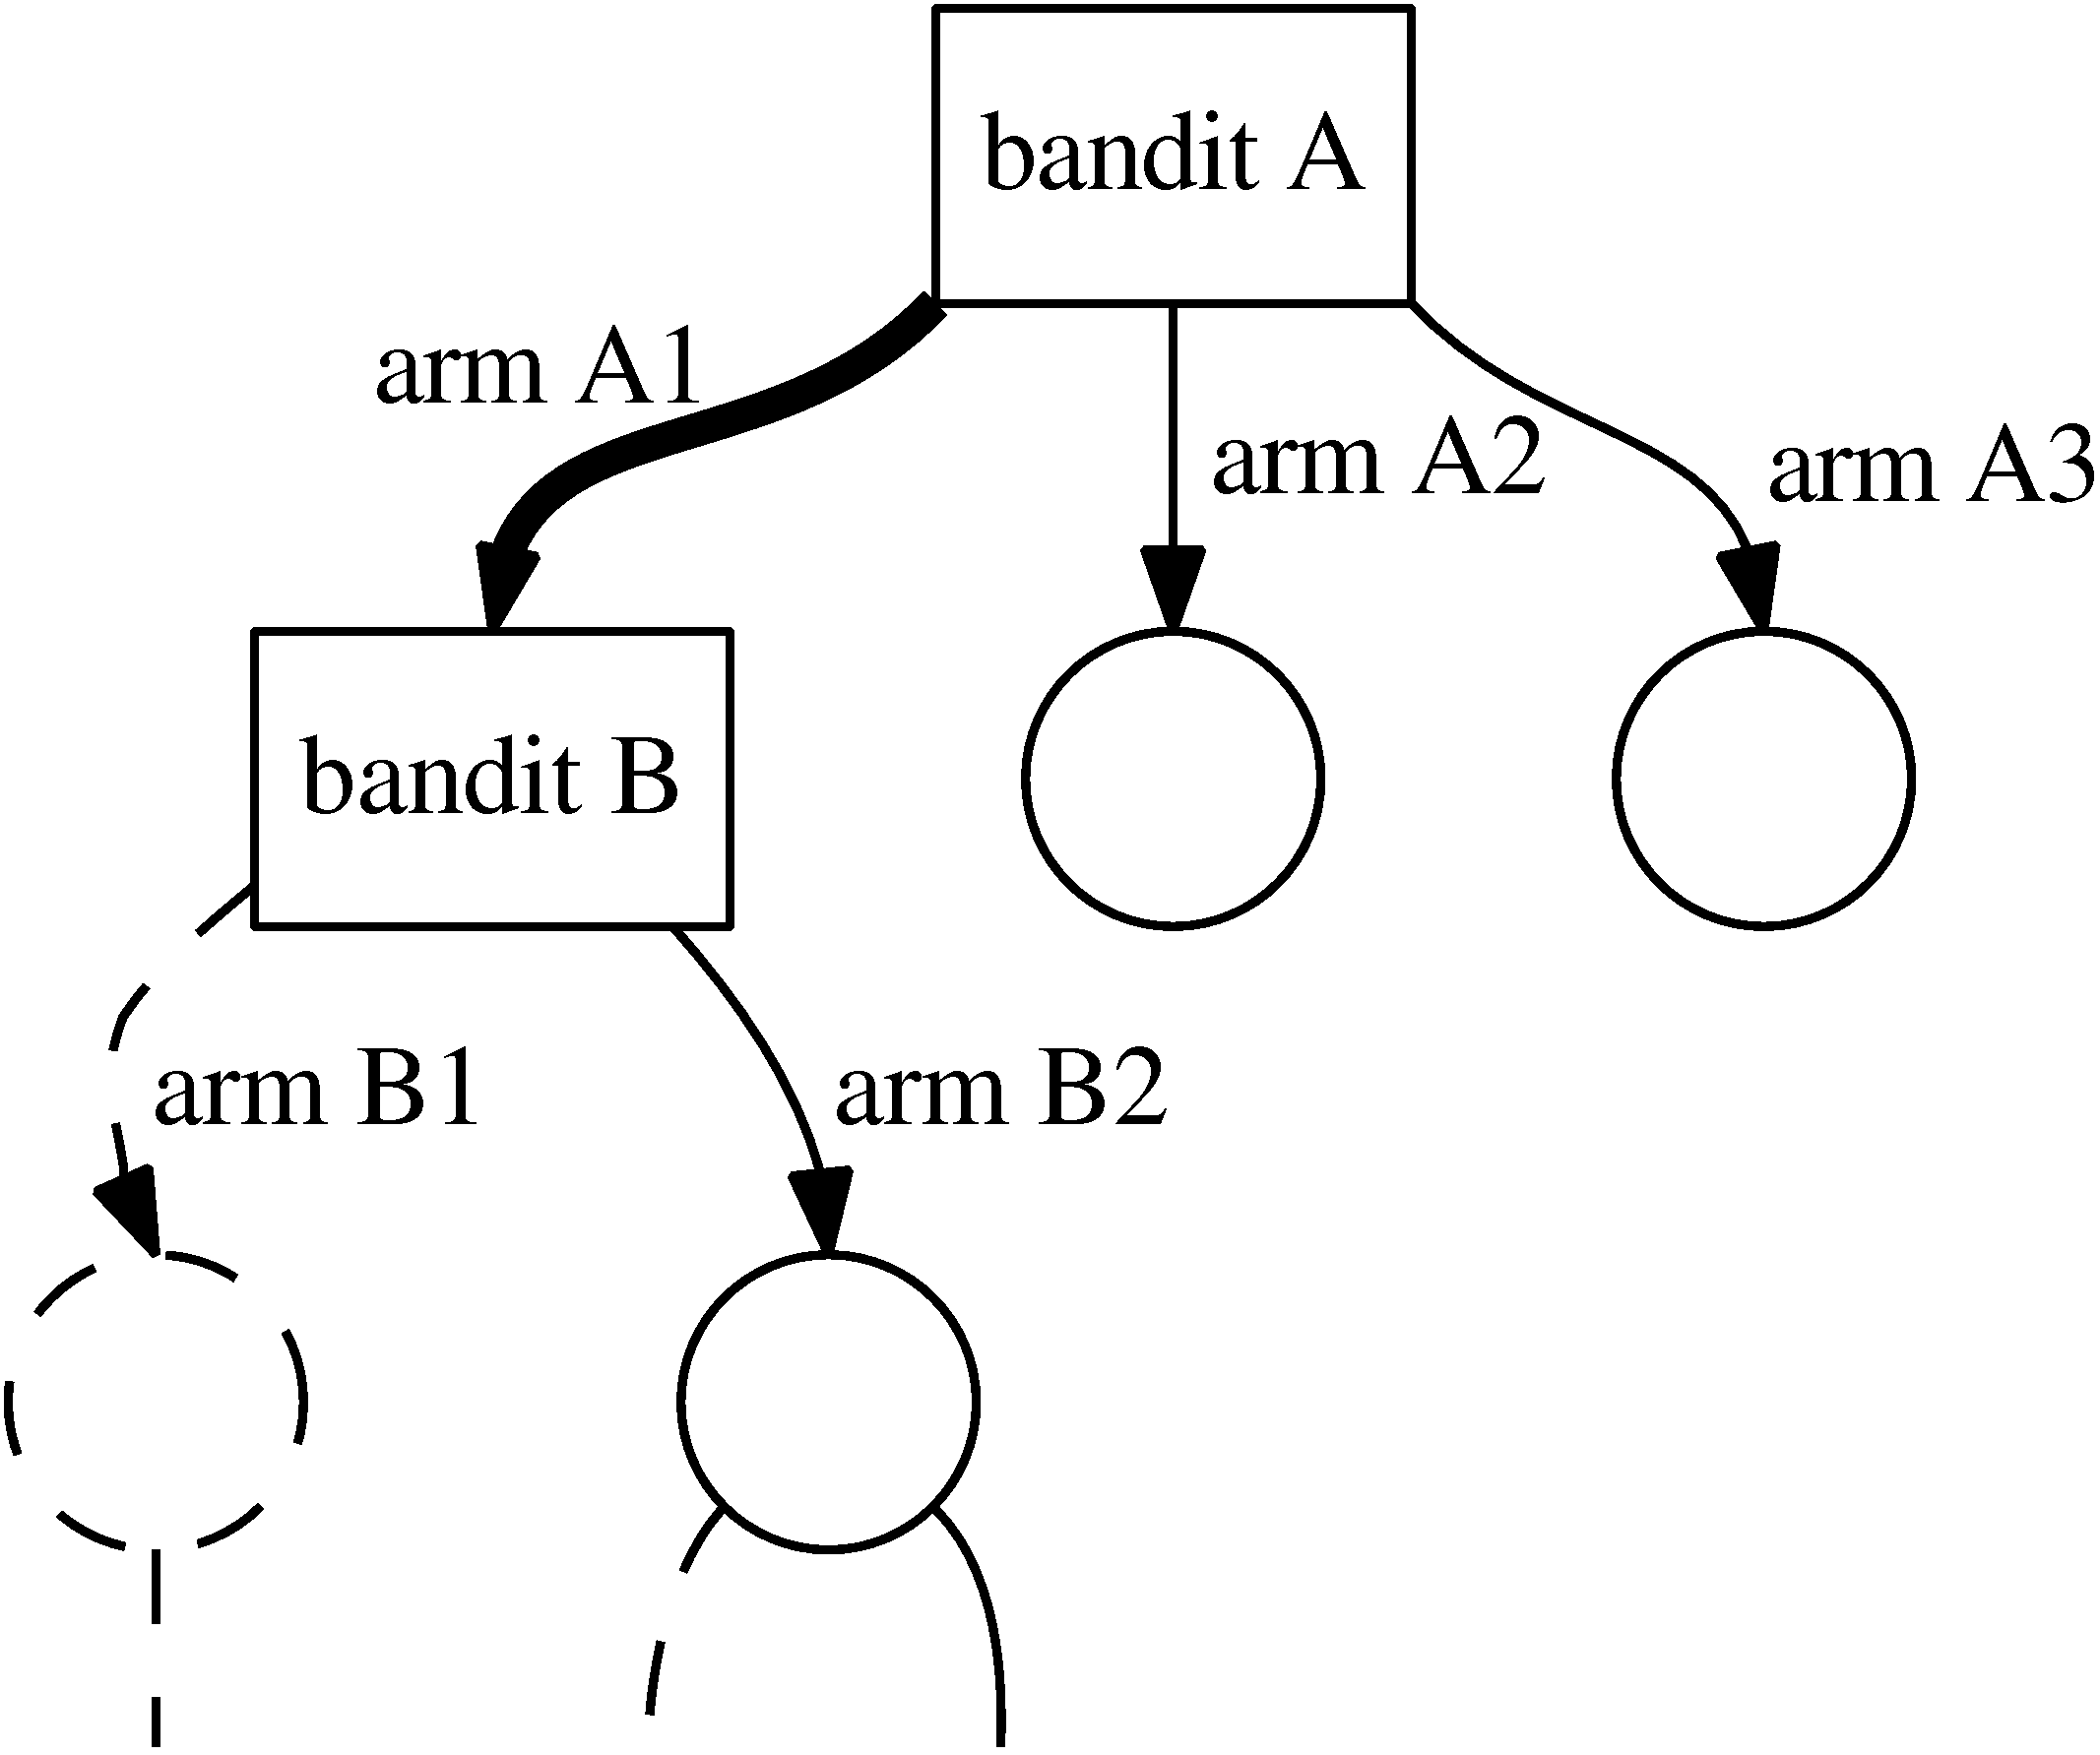
\includegraphics[scale=0.5]{figs/bandit_cascade.png}
    \end{center}


\end{frame}

\begin{frame}
    \frametitle{UCB en pratique}
    \begin{itemize}
        \item Ajout d'un paramètre $p$ de contrôle de l'exploration:
            $$ \hat{\mu}_{i,t-1} + {\color{blue}p} \sqrt{\frac{\log(t)}{T_i(t-1)}} $$
        \item Ajout de connaissances a priori $C_i(t)$:
            $$ \hat{\mu}_{i,t-1} + p \sqrt{\frac{\log(t)}{T_i(t-1)}} + {\color{blue} C_i(t)} $$
    \end{itemize}
    
\end{frame}

\begin{frame}
    \frametitle{Améliorations}
    \begin{itemize}
        \item Ordonner les bras du bandit
        \itemSo limiter le nombre de bras explorés
        \item Ajouter de connaissances expertes \cite{chaslot2009adding}
        \itemSo modifier la formule de bandit ou la distribution de probabilité pour l'évaluation
        \item Rapide Action Value Estimation (RAVE) \cite{gelly2007combining}
        \itemSo prendre en compte le fait qu'inverser la séquence de coup peut donner le même résultat
        \item ...
    \end{itemize}
    
\end{frame}



\frame{
  \frametitle{Échelle de niveau}

\centering

\begin{tikzpicture}

    %vertical lines
    \draw [->, very thick] (0,-0.5) -- (0,5.5);
    \draw [->, very thick] (2,4) -- (2,5.5);

    %horizontal lines
    \foreach \x in {0,1,2,3,4}
        \draw [thick] (-3pt, \x) -- (3pt, \x);

    \draw [dashed] (0,4) -- (2,4);

    %nodes
    \draw (0,0) node[left=3pt] {$30$ kyu};
    \draw (0,1) node[left=3pt] {$20$ kyu};
    \draw (0,2) node[left=3pt] {$10$ kyu};
    \draw (0,2.75) node[left=3pt] {$1$ kyu};
    \draw (0,3.25) node[left=3pt] {$1$ dan};
    \draw (0,4) node[left=3pt] {$6$ dan};
    \draw (2,4) node[right=3pt] {$1$ dan};
    \draw (0,5.5) node[left=3pt] {$9$ dan};
    \draw (2,5.5) node[right=3pt] {$9$ dan};

    \draw (0,6.5) node[] {\textbf{amateur}};
    \draw (2,6.5) node[] {\textbf{pro}};

    \draw (-3,0.5) node[] {débutant};
    \draw (-3,2) node[] {moyen};
    \draw (-3,3) node[] {fort};
    \draw (-3,4) node[] {très fort};
    \draw (-3,5.5) node[] {meilleur};

    \draw (4,2) node[rectangle,fill=black] {} node[right=3pt] {GNU Go};
    \draw (4,4) node[rectangle,fill=red] {} node[right=3pt,color=red] {MoGo};

\end{tikzpicture}
}

\frame{
  \frametitle{Première victoire en 9x9 en tant que joueur noir}

  \begin{columns}
      \begin{column}{0.6\textwidth}
          \begin{itemize}
              \item programme: MoGoTW
              \itemSo MCTS avec de nombreuses améliorations
              \itemSo 32 machines de 8 coeurs
              \item adversaire: C.-H. Chou (pro 9 dan)
          \end{itemize}
      \end{column}
      \begin{column}{0.4\textwidth} 
          \begin{center}
              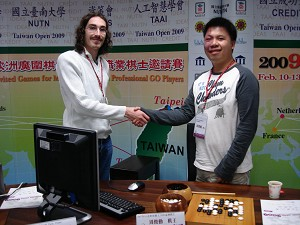
\includegraphics[width=1\textwidth]{figs/mogo99win.jpg}
          \end{center}
      \end{column}
  \end{columns}


}

\section{Conclusion}

\frame{
  \frametitle{Alphago}

  TODO principe en 1 slide
}

\frame{
  \frametitle{Échelle de niveau}

\centering

\begin{tikzpicture}

    %vertical lines
    \draw [->, very thick] (0,-0.5) -- (0,5.5);
    \draw [->, very thick] (2,4) -- (2,5.5);

    %horizontal lines
    \foreach \x in {0,1,2,3,4}
        \draw [thick] (-3pt, \x) -- (3pt, \x);

    \draw [dashed] (0,4) -- (2,4);

    %nodes
    \draw (0,0) node[left=3pt] {$30$ kyu};
    \draw (0,1) node[left=3pt] {$20$ kyu};
    \draw (0,2) node[left=3pt] {$10$ kyu};
    \draw (0,2.75) node[left=3pt] {$1$ kyu};
    \draw (0,3.25) node[left=3pt] {$1$ dan};
    \draw (0,4) node[left=3pt] {$6$ dan};
    \draw (2,4) node[right=3pt] {$1$ dan};
    \draw (0,5.5) node[left=3pt] {$9$ dan};
    \draw (2,5.5) node[right=3pt] {$9$ dan};

    \draw (0,6.5) node[] {\textbf{amateur}};
    \draw (2,6.5) node[] {\textbf{pro}};

    \draw (-3,0.5) node[] {débutant};
    \draw (-3,2) node[] {moyen};
    \draw (-3,3) node[] {fort};
    \draw (-3,4) node[] {très fort};
    \draw (-3,5.5) node[] {meilleur};

    \draw (4,2) node[rectangle,fill=black] {} node[right=3pt] {GNU Go};
    \draw (4,4) node[rectangle,fill=black] {} node[right=3pt] {MoGo};
    \draw (4,5.5) node[rectangle,fill=red] {} node[right=3pt,color=red] {AlphaGo};

\end{tikzpicture}
}

\frame{
  \frametitle{Autres applications}

  \begin{itemize}
      \item jeux:
  \begin{itemize}
      \item jeux de plateaux
      \itemSo Havannah \cite{ewals2012playing}, Hex \cite{arneson2009mohex}, ...
      \item jeux vidéos
      \itemSo Ms. Pac-Man \cite{pepels2014real}, ...
      \item jeux non déterministes
      \itemSo Poker \cite{rubin2011computer}, Magic \cite{ward2009monte}, ...
  \end{itemize}
          \item autre:
  \begin{itemize}
      \item couplage de graphe \cite{pinheiro2017geometric}
      \item planification \cite{nakhost2009monte}
      \item calcul de transformée de Fourier rapide \cite{de2009bandit}
      \item ...
  \end{itemize}
  \end{itemize}
}

\frame{
  \frametitle{Conclusion}

  \begin{center}
  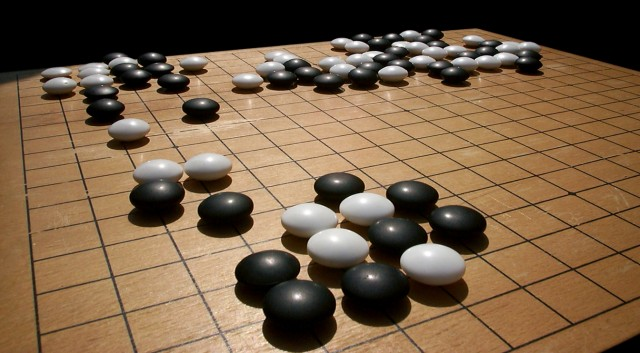
\includegraphics[width=0.3\textwidth]{figs/go-intro.jpg}
  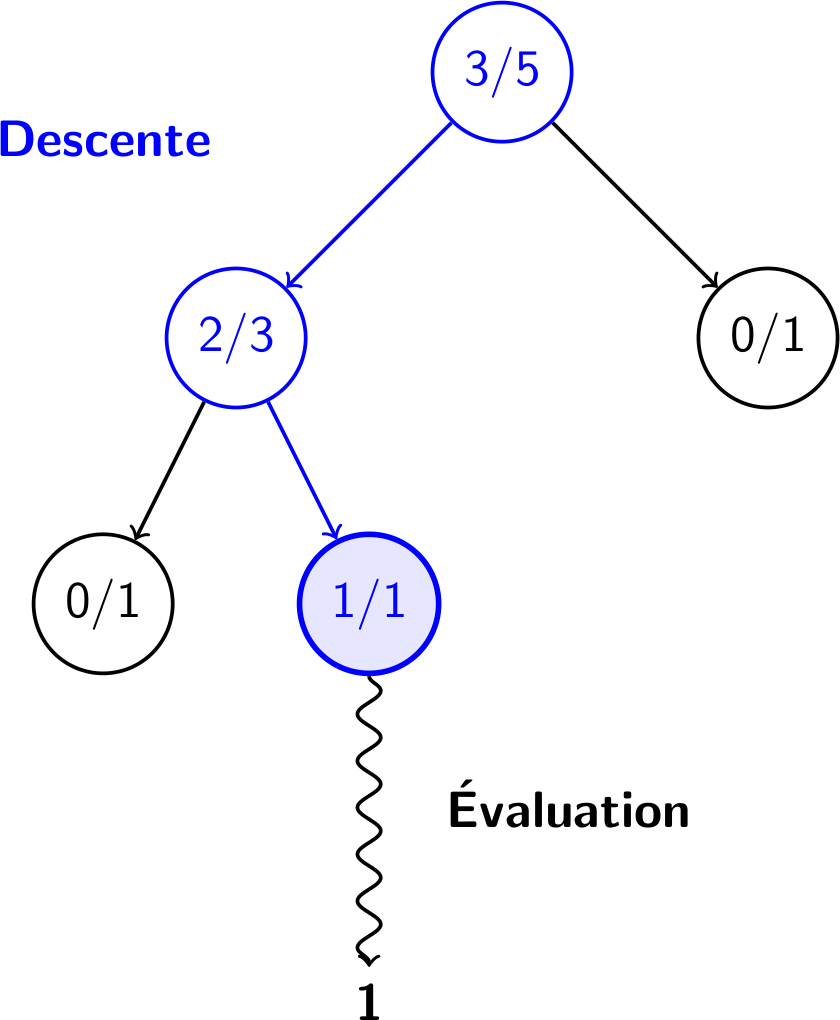
\includegraphics[width=0.25\textwidth]{figs/mcts_exemple.png}
  \end{center}

  \begin{itemize}
      \item méthode d'exploration d'arbre \red{déséquilibré}
      \item a permis de battre les meilleurs humains au jeu de \textbf{Go}
      \item méthode \red{générique} pouvant être appliqué à d'autres problèmes
  \end{itemize}
  TODO image
}

\begin{frame}[allowframebreaks]
    \frametitle{Références}
    \bibliographystyle{apalike}
    \bibliography{mcts.bib}
\end{frame}





%\frame{
%  \frametitle{Exemple borne}
%
%\centering
%
%\begin{tikzpicture}
%
%    \node [circle,draw] (a) at (0,0) {a};
%    \node [circle,draw] (b) at (3,0) {b};
%    \node [circle,draw] (c) at (6,0) {c};
%    \node [circle,draw] (d) at (0,-4) {d};
%    \node [circle,draw] (e) at (-3,-4) {e};
%
%    \draw [dashed] (a) -- (b) node [pos=0.5]{\textbf{3}};
%    \draw [dashed] (a) -- (d) node [pos=0.3]{\textbf{4}};
%    \draw [dashed] (a) -- (e) node [pos=0.5]{\textbf{5}};
%  
%    \draw [dashed] (b) -- (c) node [pos=0.5]{\textbf{3}};
%    \draw [dashed] (b) -- (d) node [pos=0.3]{5};
%    \draw [dashed] (b) -- (e) node [pos=0.3]{7};
%  
%    \draw [dashed] (c) -- (d) node [pos=0.5]{\textbf{7}};
%    \draw [dashed] (c) -- (e) node [pos=0.3]{10};
%  
%    \draw [dashed] (d) -- (e) node [pos=0.5]{\textbf{3}};
%\end{tikzpicture}
%
%    \begin{block}{Calcul de la borne}
%        trajet déjà effectué = $\emptyset$
%
%        $(\underbrace{3+4}_{a}+\underbrace{3+3}_{b}+\underbrace{3+7}_{c}+\underbrace{3+4}_{d}+\underbrace{3+5}_{e})/2=19$
%    \end{block}
%
%}

\fi
\end{document}
